

\chapter[Proof techniques I]{Proof techniques I --- Standard methods}
\label{ch:proof1}

{\em Love is a snowmobile racing across the tundra and then suddenly it %
 flips over, pinning you underneath. At night, the \index{weasels, ice} %
 ice weasels come. --Matt Groening} 

\section{Direct proofs of universal statements}
\label{sec:direct}

If you form the product of 4 consecutive numbers, the result will be one 
less than a perfect square.  Try it!

\[ 1 \cdot 2 \cdot 3 \cdot 4 = 24 = 5^2 - 1 \]

\[ 2 \cdot 3 \cdot 4 \cdot 5 = 120 = 11^2 - 1 \]

\[ 3 \cdot 4 \cdot 5 \cdot 6 = 360 = 19^2 - 1 \]

It always works!

The three calculations that we've carried out above constitute an
inductive argument in favor of the result.  If you like we can try 
a bunch of further examples,

\[ 13 \cdot 14 \cdot 15 \cdot 16 = 43680 = 209^2 - 1 \]

\[ 14 \cdot 15 \cdot 16 \cdot 17 = 571200 = 239^2 - 1 \]

\noindent but really, no matter how many examples we produce, we haven't 
{\em proved} the statement --- we've just given evidence.


Generally, the first thing to do in proving a universal statement like 
this is to rephrase it as a conditional.  The resulting statement is a 
\index{universal conditional statement}\emph{Universal Conditional Statement} 
or a UCS.  The reason for taking 
this step is that the \emph{hypotheses} will then be clear -- they form 
the antecedent of the UCS.  So, while you won't have really made any 
progress in the proof by taking this advice, you will at least know what tools
you have at hand.  Taking the example we started with, and rephrasing 
it as a UCS we get

\[ \forall a,b,c,d \in \Integers, (\mbox{a,b,c,d  consecutive}) 
\implies \exists k \in \Integers, a{\cdot}b{\cdot}c{\cdot}d = k^2 -1 
\]

The antecedent of the UCS is that $a,b,c$ and $d$ must be 
{\em consecutive}.  By concentrating our attention on what it 
means to be consecutive, we should quickly realize that the original
way we thought of the problem involved a red herring.  We don't need 
to have variables for all four numbers; because they are consecutive, 
$a$ uniquely determines the other three.  Finally we have a version 
of the statement that we'd like to prove that should lend itself
to our proof efforts.

\begin{thm} 
\[ \forall a \in \Integers, \exists k \in \Integers, 
a(a+1)(a+2)(a+3) = k^2 - 1. \]
\end{thm}

In this simplistic example, the only thing we need to do is come 
up with a value for $k$ given that we know what $a$ is.  In other 
words, a ``proof'' of this statement involves doing some algebra.

Without further ado\ldots

\begin{proof}
Suppose that $a$ is a particular but arbitrarily chosen 
integer.  Consider the product of the 4 consecutive integers, $a$, 
$a+1$, $a+2$ and $a+3$.  We would like to show that this product is 
one less than the square of an integer $k$.  Let $k$ be $a^2+3a+1$.  

First, note that 

\[  a(a+1)(a+2)(a+3) = a^4 + 6a^3 + 11a^2 + 6a. \]

Then, note that

\begin{gather*} 
k^2 - 1 = (a^2 + 3a +1)^2 - 1 \\
= (a^4  + 6a^3 + 11a^2 + 6a + 1) - 1 \\
= a^4 + 6a^3 + 11a^2 + 6a. 
\end{gather*}

\end{proof} 

Now, if you followed the algebra above, (none of which was particularly 
difficult) the proof stands as a completely valid argument showing the 
truth of our proposition, but this is \emph{very} unsatisfying!  All 
the real work was concealed in one stark little sentence:
``Let $k$ be $a^2+3a+1$.''   Where on Earth did that particular value 
of $k$ come from?  The answer to that question should hopefully 
convince you that there is a huge difference between \emph{devising} 
a proof and \emph{writing} one.  A good proof can sometimes be
somewhat akin to a good demonstration of magic, a magician doesn't 
reveal the inner workings of his trick, neither should a mathematician 
feel guilty about leaving out some of the details behind the work!  
Heck, there are plenty of times when you just have to \emph{guess} 
at something, but if your guess works out, you can write
a perfectly correct proof.  

In devising the proof above, we multiplied out the consecutive numbers 
and then realized that we'd be done if we could find a polynomial in 
$a$ whose square was $a^4  + 6a^3 + 11a^2 + 6a + 1$.  Now, obviously, 
we're going to need a quadratic polynomial, and because the leading 
term is $a^4$ and the constant term is $1$, it should be of the form 
$a^2 + ma + 1$.  Squaring this gives $a^4 + 2ma^3 + (m^2+2)a^2 + 2ma + 1$ 
and comparing that result with what we want, we pretty quickly realize 
that $m$ had better be 3.  So it wasn't magic after all!

This seems like a good time to make a comment on polynomial arithmetic.
\index{polynomial multiplication}  
Many people give up (or go searching for a computer algebra system) 
when dealing with products of anything bigger than binomials.  This 
is a shame because there is an easy method using a table for performing 
such multiplications.  As an example, in devising the previous proof we 
needed to form the product $a(a+1)(a+2)(a+3)$, now we can use the
distributive law or the infamous F.O.I.L rule to multiply pairs of these, 
but we still need to multiply $(a^2+a)$ with $(a^2+5a+6)$.  Create a 
table that has the terms of these two polynomials as its row and column 
headings.

\begin{center}
\begin{tabular}{c|ccc}
      & \rule{3pt}{0pt} $a^2$ \rule{3pt}{0pt}  & \rule{3pt}{0pt}  $5a$ \rule{3pt}{0pt}  & \rule{3pt}{0pt}  $6$  \rule{3pt}{0pt} \\ \hline
$a^2$ &         &      & \\
$a$   &         &      & \\
\end{tabular}
\end{center}

Now, fill in the entries of the table by multiplying the corresponding 
row and column headers.

\begin{center}
\begin{tabular}{c|ccc}
      &  \rule{3pt}{0pt}   $a^2$ \rule{3pt}{0pt}  & \rule{3pt}{0pt}  $5a$  \rule{3pt}{0pt}   &  \rule{3pt}{0pt} $6$  \rule{3pt}{0pt} \\ \hline
$a^2$ &   $a^4$ & $5a^3$ & $6a^2$ \\
$a$   &   $a^3$ & $5a^2$ & $6a$ \\
\end{tabular}
\end{center}

Finally add up all the entries of the table, combining any like terms.

You should note that the F.O.I.L rule is just a mnemonic for the case when 
the table has 2 rows and 2 columns.

Okay, let's get back to doing proofs.  We are going to do a lot of
proofs involving the concepts of elementary number theory so, as a 
convenience, all of the definitions that were made in Chapter~\ref{ch:intro}
are gathered together in Table~\ref{tab:defs}.

\begin{tabular}{l}
\rule{12pt}{0pt} Even \\
\framebox{\begin{minipage}{.8\textwidth}%
\rule[-6pt]{0pt}{20pt} $\forall n \in \Integers$, \\
\centerline{\rule[-6pt]{0pt}{20pt}$n$ is even \rule{6pt}{0pt} $\iff$ \rule{6pt}{0pt} $\exists  k \in \Integers, \; n = 2k$} \end{minipage} }\\
\rule{12pt}{0pt} Odd \\
\framebox{\begin{minipage}{.8\textwidth}%
\rule[-6pt]{0pt}{20pt} $\forall n \in \Integers$, \\
\centerline{\rule[-6pt]{0pt}{20pt}$n$ is odd \rule{6pt}{0pt} $\iff$ \rule{6pt}{0pt} $\exists
 k \in \Integers, \; n = 2k+1$} \end{minipage} }\\
\rule{12pt}{0pt} Divisibility\\
\framebox{\begin{minipage}{.8\textwidth}%
\rule[-6pt]{0pt}{20pt} $\forall n \in \Integers , \forall \quad d>0 \in \Integers$, \\
\centerline{\rule[-6pt]{0pt}{20pt}$d \divides n$  \rule{6pt}{0pt} $\iff$ \rule{6pt}{0pt} $\exists
 k \in \Integers, \; n = kd$} \end{minipage} } \\
\rule{12pt}{0pt} Floor\\
\framebox{\begin{minipage}{.8\textwidth}%
\rule[-6pt]{0pt}{20pt} $\forall x \in \Reals$, \\
\centerline{\rule[-6pt]{0pt}{20pt}$y = \lfloor x \rfloor$  \rule{6pt}{0pt} $\iff$ \rule{6pt}{0pt} 
$ y \in \Integers \, \; \land \, \; y \leq x < y+1$} \end{minipage} }\\
\rule{12pt}{0pt} Ceiling\\
\framebox{\begin{minipage}{.8\textwidth}%
\rule[-6pt]{0pt}{20pt} $\forall x \in \Reals$, \\
\centerline{\rule[-6pt]{0pt}{20pt}$y = \lceil x \rceil$  \rule{6pt}{0pt} $\iff$ \rule{6pt}{0pt} 
$ y \in \Integers \, \; \land \, \; y-1 < x \leq y$} \end{minipage} }\\
\rule{12pt}{0pt} Quotient-remainder theorem, Div and Mod\\
\framebox{\begin{minipage}{.8\textwidth}%
\rule[-6pt]{0pt}{20pt}$\forall n, d>0 \in \Integers$,\\
\centerline{\rule[-6pt]{0pt}{20pt}$\exists \mbox{!} q,r \in \Integers, \; n = qd + r \, \; \land \, \; 0 \leq r < d $} 
\rule[-6pt]{0pt}{20pt}\centerline{$n \; \mbox{div} \; d = q$} \newline
\rule[-6pt]{0pt}{20pt}\centerline{$n \; \mbox{mod} \; d = r$} 
\end{minipage} }\\
\rule{12pt}{0pt} Prime\\
\framebox{\begin{minipage}{.8\textwidth}%
\rule[-6pt]{0pt}{20pt}$\forall \, p \, \in \Integers$\\
\rule[-6pt]{0pt}{20pt}\centerline{$p$ is prime \rule{6pt}{0pt}%
$\iff$ \rule{60pt}{0pt} }
\rule[-6pt]{0pt}{12pt}\centerline{\rule{30pt}{0pt} $(p>1) \quad \land \quad (\forall x,y \in \Integers^+, \; p=xy \; \implies \; x=1 \, \lor \,  y=1)$} 
\end{minipage} }\\
\end{tabular}



\clearpage 

In this section we are concerned with 
\index{direct proofs}direct proofs of universal statements.  
Such statements come in two flavors -- those that appear to involve 
conditionals, and those that don't:

\begin{quote} Every prime greater than two is odd.
\end{quote}

versus

\begin{quote} For all integers $n$, if $n$ is a prime greater than two, then $n$ is odd.
\end{quote}

These two forms can readily be transformed one into the other, so 
we will always concentrate on the latter.  A direct proof of a UCS
always follows a form known as 
\index{generalizing from the generic particular}
``generalizing from the generic particular.''
We are trying to prove that $\forall x \in U, P(x) \implies Q(x)$.  
The argument (in skeletal outline) will look like:
\medskip

\begin{center}
\begin{tabular}{|c|} \hline
\rule{16pt}{0pt}\begin{minipage}{.75\textwidth}
\rule{0pt}{20pt} {\em Proof:} Suppose that $a$ is a particular but arbitrary element of $U$ such 
that $P(a)$ holds.

\begin{center}
$\vdots$
\end{center}

Therefore $Q(a)$ is true. \newline
Thus we have shown that for all $x$ in $U$, $P(x) \implies Q(x)$.\newline
\rule{0pt}{0pt} \hspace{\fill} Q.E.D. \rule[-10pt]{0pt}{16pt}
\end{minipage} \rule{16pt}{0pt} \\ \hline
\end{tabular}
\end{center}
\medskip

Okay, so this outline is pretty crappy.  It tells you how to start and 
end a direct proof, but those obnoxious dot-dot-dots in the middle are 
where all the real work has to go.  If I could tell you (even in outline) 
how to fill in those dots, that would mean mathematical proof isn't really 
a very interesting activity to engage in.  Filling in those dots will 
sometimes (rarely) be obvious, more often it will be extremely challenging; 
it will require great creativity, loads of concentration, you'll call on 
all your previous mathematical experiences, and you will most likely
experience a certain degree of anguish.  Just remember that your sense 
of accomplishment is proportional to the difficulty of the puzzles you 
attempt.  So let's attempt another\ldots

In Table~\ref{tab:defs} one of the very handy notions defined is that 
of the \emph{floor} of a real number. 

\[ y = \lfloor x \rfloor \; \iff \; (y \in \mathbb Z \; \land \; y \leq x < y+1).\]

There is a sad tendency for people to apply old rules in new situations 
just because of a chance similarity in the notation.  The brackets used 
in notating the floor function look very similar to ordinary parentheses, 
so the following ``rule'' is often proposed

\[ \lfloor x + y \rfloor = \lfloor x \rfloor + \lfloor y \rfloor \]

\begin{exer} 
Find a counterexample to the previous ``rule.''
\end{exer}

What is (perhaps) surprising is that if one of the numbers involved is an
integer then the ``rule'' really works.

\begin{thm}
\[ \forall x \in \Reals, \, \forall n \in \Integers, \, 
\lfloor x + n \rfloor = \lfloor x \rfloor + \lfloor n \rfloor \]
\end{thm}

Since the floor of an integer {\em is} that integer, we could restate this
as $ \lfloor x + n \rfloor = \lfloor x \rfloor +  n$. 

Now, let's try rephrasing this theorem as a UCS:  If $x$ is a real number
and $n$ is an integer, then $\lfloor x + n \rfloor = \lfloor x \rfloor +  n$.
This is bad \ldots it appears that the only hypotheses that we can use
involve what kinds of numbers $x$ and $n$ are --- our hypotheses aren't
particularly potent.  Your next most useful allies in constructing proofs
are the definitions of the concepts involved.  The quantity 
$\lfloor x \rfloor$ appears in the theorem, let's make
use of the definition:

\[ a = \lfloor x  \rfloor \; \iff \; a \in \Integers \; \, 
\land \; \, a \leq x < a+1. \]

The only other floor function that appears in the statement of the theorem
(perhaps even more prominently) 
is $\lfloor x + n\rfloor$, here, the definition gives us
 
\[ b = \lfloor x + n \rfloor \; \iff \; 
b \in \Integers \; \, \land \; \, b \leq x + n < b+1. \]

These definitions are our only available tools so we'll certainly \emph{have}
to make use of them, and it's important to notice that that is a good thing;
the definitions allow us to work with something well-understood 
(the inequalities that appear within them) rather than with something 
new and relatively suspicious (the floor notation).  Putting the proof 
of this statement together is an exercise in staring at the two definitions 
above and noting how one can be converted into the other.  It is also a 
testament to the power of \emph{naming} things.

\begin{proof}
Suppose that $x$ is a particular but arbitrary real number 
and that $n$ is a particular but arbitrary integer.  Let 
$a = \lfloor x \rfloor$.  By the definition of the floor function 
it follows that $a$ is an integer and $a \leq x < a+1$.  By adding 
$n$ to each of the parts of this inequality
we deduce a new (and equally valid) inequality, $a+n \leq x+n < a+n+1$.
Note that $a+n$ is an integer and the inequality above together with
this fact constitute precisely the definition of 
$a + n = \lfloor x + n \rfloor$.  Finally, recalling that 
$a = \lfloor x \rfloor$ (by assumption), and rewriting, we obtain the
desired result

\[ \lfloor x + n \rfloor = \lfloor x \rfloor + n. \]

\end{proof} 

As we've seen in the examples presented in this section, coming up
with a proof can sometimes involve a bit of ingenuity. But, sometimes, 
there is a ``follow your nose'' sort of approach that will
allow you to devise a valid argument without necessarily displaying
any great leaps of genius!  Here are a few pieces
of advice about proof-writing:

\begin{itemize}
\item Before anything else, determine precisely what hypotheses you
can use.
\item Jot down the definitions of {\em anything} in the statement of 
the theorem.
\item There are 26 letters at your disposal (and even more if you know
Greek) (and you can always throw on subscripts!) don't be stingy with
letters.  The nastiest mistake you can make is to use the same variable
for two different things.
\item Please write a rough draft first.  Write two drafts!  Even if you
can write beautiful, lucid prose on the first go around, it won't fly
when it comes to organizing a proof.
\item The statements in a proof are supposed to be logical statements.
That means they should be Boolean (statements that are either true or false).
An algebraic expression all by itself doesn't count, an inequality or an 
equality does.  
\item Don't say ``if'' when you mean ``since.''  Really!  If you start a
proof about rational numbers like so:

\begin{quote}
{\em Proof:} Suppose that $x$ is a particular but arbitrary rational number.
If $x$ is a rational number, it follows that \ldots
\end{quote}

\noindent people are going to look at you funny.  What's the point of 
{\em supposing}
that $x$ is rational, then acting as if you're in doubt of that fact by
writing ``if''?   You mean ``since.''
\item Mark off the beginning and the end of your proofs as a hint to your
readers.  In this book we start off a proof by writing {\em Proof:} in 
italics and we end every proof with the abbreviation 
\index{quod erat demonstrandum}
Q.E.D.\footnote{{\em Quod erat demonstrandum} or ``(that) which was to 
be demonstrated.'' some authors prefer placing a small rectangle at 
the end of their proofs, but Q.E.D. seems more pompous.}
\end{itemize}

\newpage

We'll close this section with a word about axioms.  The axioms in any
given area of math are your most fundamental tools.  Axioms don't
need to be proved -- we are supposed to just accept them!  A very common 
problem for beginning proofwriters is telling the difference between statements
that are axiomatic and statements that require some proof.  For instance, in the
exercises for this section there is a problem that asks us to prove that the sum of
two rational numbers is rational.  Doesn't this seem like it might be one of
the axioms of rational numbers?  Is it really something that {\em can} be proved?
Well, we know how the process of adding rational numbers works: we put the
fractions over a common
denominator and then just add numerators.  Do you see how adding fractions really rests
on our ability to add the numerators (which are integers).  So, in doing that exercise you
can use the fact (indeed, you'll need to use the fact) that the sum of two integers is an integer.
So how about {\em that} statement?  Is it necessary to prove that adding integers produces 
an integer?  As a matter of fact it {\em is} necessary since the structure of the integers 
rests on a foundation known as the Peano axioms for the naturals -- and the Peano axioms
{\em don't} include one that guarantees that the sum of two naturals is also a natural.  If you
are tempted to trace this whole thing back, to ``find out how deep the rabbit hole goes,'' I commend
you.   But, if you just want to be able to get on with doing your homework problems, I sympathize 
with that sentiment too.  Let's agree that integers behave the way we've come to expect -- if 
you add or multiply integers the result will be an integer. 

\newpage

\noindent{\large \bf Exercises --- \thesection\ }

\begin{enumerate}
\item Every prime number greater than 3 is of one of the two forms
$6k+1$ or $6k+5$.  What statement(s) could be used as hypotheses in
proving this theorem?

\hint{

\vfill

Fill in the blanks:
\begin{itemize}
\item $p$ is a \underline{\rule{1.5in}{0in}} number, and
\item $p$ is greater than \underline{\rule{1in}{0in}}.
\end{itemize}

\vfill

}

\item Prove that 129 is odd.

\hint{

\vfill

\rule{12pt}{0pt} All you have to do to show that some number is odd, is produce the integer $k$ that the definition
of ``odd'' says has to exist.  Hint: the same number could be used to prove that $128$ is even.

\vfill

}

\item Prove that the sum of two rational numbers is a rational number.

\hint{

\vfill

\rule{12pt}{0pt} You want to argue about the sum of two generic rational numbers. Maybe call them $a/b$ and $c/d$. The definition of ``rational number'' then tells you that $a$, $b$, $c$ and $d$ are integers and that neither $b$ nor $d$ are zero. You add these generic rational numbers in the usual way -- put them over a common denominator and then add the numerators. One possible common denominator is $bd$, so we can express the sum as $(ad+bc)/(bd)$.  You can finish off the argument from here: you need to show that this expression for the sum satisfies the definition of a rational number (quotient of integers w/ non-zero denominator). Also, write it all up a bit more formally\ldots

\vfill

}

\hintspagebreak

\item Prove that the sum of an odd number and an even number is odd.


\hint{

\vfill

\begin{proof}
Suppose that $x$ is an odd number and $y$ is an even number.  Since $x$ is odd there is an 
integer $k$ such that $x=2k+1$.  Furthermore, since $y$ is even, there is an integer $m$ such that
$y=2m$.  By substitution, we can express the sum $x+y$ as $x+y = (2k+1) + (2m) = 2(k+m) + 1$.
Since $k+m$ is an integer (the sum of integers is an integer) it follows that $x+y$ is odd.
\end{proof}

\vfill

}

\item Prove that if the sum of two integers is even, then so is their
difference.

\hint{

\vfill

Hint: If we write $x+y$ for the sum of two integers that is even (so $x+y = 2k$ for some integer $k$), then we could subtract \underline{\rule{1in}{0in}} from it in order to obtain $x-y$. Once you fill in that blank properly the flow of the argument should become apparent to you.

\vfill

}

\item Prove that for every real number $x$, $\frac{2}{3} < x < \frac{3}{4} \; \implies \; \lfloor 12x \rfloor = 8$.

\hint{

\vfill

Begin your proof like so:

``Suppose that $x$ is a real number such that $\frac{2}{3} < x < \frac{3}{4}$.''

You need to multiply all three parts of the inequality by something in order to ``clear'' the fractions.
What should that be?


The definition for the floor of $12x$ will be satisfied if $8 \leq 12x < 9$ but unfortunately the work done 
previously will have deduced that $8 < 12x < 9$ is true.  Don't just gloss over this discrepancy.  Explain why
one of these inequalities is implied by the other.

\vfill

}

\hintspagebreak

\item Prove that if $x$ is an odd integer, then $x^2$ is of the form
$4k+1$ for some integer $k$.

\hint{

\vfill

\rule{12pt}{0pt} You may be tempted to write ``Since x is odd, it can be expressed as $x = 2k+1$ where $k$ is an integer.'' This is slightly wrong since the variable $k$ is already being used in the statement of the theorem. But, except for replacing $k$ with some other variable (maybe $m$ or $j$?) that {\em is} a good way to get started. From there it's really just algebra until, eventually, you'll find out what $k$ really is.

\vfill

}

\item Prove that for all integers $a$ and $b$, if $a$ is odd and $6 \divides (a+b)$, then $b$ is odd.

\hint{

\vfill

\rule{12pt}{0pt} The premise that $6 \divides (a+b)$ is a bit of a red herring (a clue that is designed to mislead).  The premise that you really need is that $a+b$ is even.  Can you deduce that from what's given?

\vfill

}

\item Prove that $\forall x\in\Reals \, x\not\in\Integers \, \implies \, \lfloor x\rfloor+\lfloor-x\rfloor=-1$.

\hint{

\vfill

\begin{proof}
Suppose that $x$ is a real number and $x\not\in\Integers$.  Let $a = \lfloor x \rfloor$.  By the definition
of the floor function we have $a \in\Integers$ and $ a \leq x < a+1$.   Since $x \not\in\Integers$ we
know that $x \neq a$ so we may strengthen the inequality to $a < x < a+1$.  Multiplying this inequality
by $-1$ we obtain $-a > -x > -a - 1$.  This inequality may be weakened to $-a > -x \geq -a - 1$.  Finally, note that (since $-a-1 \in\Integers$ and $-a = (-a-1)+1$ we
have shown that $\lfloor -x \rfloor \, = \, -a-1$.  Thus, by substitution we have $\lfloor x \rfloor+\lfloor -x \rfloor \; = \; a + (-a-1) \; = \; -1$ as desired.
\end{proof}

\vfill

}

\hintspagebreak

\item Define the \index{evenness}\emph{evenness} of an integer $n$ by:

\[ \mbox{evenness} (n) = k \; \iff \;  
 2^k \divides n \, \land \, 2^{k+1} \nmid n \]

State and prove a theorem concerning the evenness of products.

\hint{Well, the statement is that the evenness of a product is the sum of the evennesses of the factors\ldots}


\item Suppose that $a$, $b$ and $c$ are integers such that $a \divides b$
and $b \divides c$.  Prove that $a \divides c$.

\hint{
This one is pretty straightforward. Be sure to not reuse any variables. Particularly, the fact that $a \divides b$ tells us (because of the definition of divisibility) that there is an integer $k$ such that $b = ak$.  It is not okay to also use $k$ when converting the statement ``$b \divides c$.''
}

\textbookpagebreak

\item Suppose that $a$, $b$, $c$ and $d$ are integers with $a \neq c$.
Further, suppose that $x$ is a real number satisfying the equation

\[ \frac{ax+b}{cx+d} = 1. \]


\noindent Show that $x$ is rational.  Where is the hypothesis $a \neq c$
used?

\hint{Cross multiply and solve for $x$.  If you need to divide by an expression, it had 
better be non-zero!}

\item Show that if two positive integers $a$ and $b$ satisfy $a \divides b$ \emph{and}
$b \divides a$ then they are equal.

\hint{From the definition of divisibility, you get two integers $j$ and $k$, such that 
$a = jb$ and $b = ka$. Substitute one of those into the other and ask yourself what 
the resulting equation says about $j$ and $k$.  Can they be any old integers?  Or, are 
there restrictions on their values?
}

\end{enumerate}


\newpage
\section{More direct proofs}
\label{sec:more}

In creating a direct proof we need to look at our hypotheses, consider 
the desired conclusion, and develop a strategy for transforming A into B.
Quite often you'll find it easy to make several deductions from the 
hypotheses, but none of them seems to be headed in the direction of 
the desired conclusion.  The usual advice at this stage is 
\index{forwards-backwards method}
``Try working backwards from the conclusion.''
\footnote{Some people refer to this as the forwards-backwards method, since %
you work backwards from the conclusion, but also forwards from the premises, %
in the hopes of meeting somewhere in the middle.}  

There is a lovely result known as the 
\index{arithmetic-geometric mean inequality}
``arithmetic-geometric mean inequality''
whose proof epitomizes this approach.  Basically this inequality compares two
different ways of getting an ``average'' between two real numbers.  The 
\index{arithmetic mean}\emph{arithmetic mean} of two real numbers $a$ and $b$ is the one you're 
probably used to, $(a+b)/2$.   Many people just call this the ``mean''
of $a$ and $b$ without using the modifier ``arithmetic'' but as we'll
see, our notion of what intermediate value to use in between two numbers
is dependent on context.  Consider the following two sequences of numbers
(both of which have a missing entry) 

\[ 2 \rule{6pt}{0pt} 9  \rule{6pt}{0pt} 16  \rule{6pt}{0pt} 23  \rule{6pt}{0pt} \rule{12pt}{.5pt}  \rule{6pt}{0pt} 37  \rule{6pt}{0pt} 44 \]

\noindent and

\[ 3 \rule{6pt}{0pt} 6  \rule{6pt}{0pt} 12  \rule{6pt}{0pt} 24  \rule{6pt}{0pt} \rule{12pt}{.5pt}  \rule{6pt}{0pt} 96  \rule{6pt}{0pt} 192. \]

\noindent How should we fill in the blanks?

The first sequence is an 
\index{arithmetic sequence}\emph{arithmetic sequence}.  
Arithmetic sequences 
are characterized by the property that the difference between successive
terms is a constant.  The second sequence is a 
\index{geometric sequence}\emph{geometric sequence}. 
Geometric sequences have the property that the ratio of successive terms 
is a constant.  The blank in the first sequence should be filled with the 
arithmetic mean of the surrounding entries $(23+37)/2 = 30$.  The blank 
in the second sequence should be filled using the 
\index{geometric mean}geometric mean
of \emph{its} surrounding entries: $\sqrt{24\cdot 96} = 48$.

Given that we accept the utility of having two inequivalent concepts
of \emph{mean} that can be used in different contexts, it is interesting
to see how these two means compare to one another.  The 
arithmetic-geometric mean inequality states that the arithmetic mean 
is always bigger.

\[ \forall a,b \in \Reals, \rule{6pt}{0pt}  a,b \geq 0 \; \implies \;  \frac{a+b}{2} \geq \sqrt{ab} \]

In proving this statement we have little choice but to work backwards
from the conclusion because the only hypothesis we have to work with
is that $a$ and $b$ are non-negative real numbers -- which isn't a 
particularly potent tool. But what should we do?  
There isn't a good response to that 
question, we'll just have to try a bunch of different things and hope
that something will work out.  When we finally get around to writing up
our proof though, we'll have to rearrange the statements in the opposite 
order from the way they were discovered.  This means that we would 
be ill-advised to make any uni-directional inferences, we should 
strive to make biconditional connections between our statements
(or else try to intentionally make converse errors).

The first thing that appeals to your humble author is to eliminate
both the fractions and the radicals\ldots

\[ \frac{a+b}{2} \geq \sqrt{ab} \]

\[ \iff \; a+b \geq 2\sqrt{ab} \]

\[ \iff \; (a+b)^2 \geq 4ab \] 

\[ \iff \; a^2+2ab+b^2 \geq 4ab \] 

One of the steps above involves squaring both sides of an inequality.
We need to ask ourselves if this step is really reversible.  In other
words, is the following conditional true?

\[ \forall x,y \in \Rnoneg, \, \; 
x \geq y \; \implies \sqrt{x} \geq \sqrt{y} \]

\begin{exer} 
Provide a justification for the previous implication.
\end{exer}

What should we try next?  There's really no good justification for
this but experience working with quadratic polynomials either in 
equalities or inequalities leads most people to try ``moving everything
to one side,'' that is, manipulating things so that one side of the 
equation or inequality is zero.

\[  a^2+2ab+b^2 \geq 4ab \] 

\[ \iff \; a^2-2ab+b^2 \geq 0 \] 

Whoa!  We're done!  Do you see why?  If not, I'll give you one
hint:  the square of any real number is greater than or equal to
zero.

\begin{exer} 
Re-assemble all of the steps taken in the previous few paragraphs
into a proof of the arithmetic-geometric mean inequality.
\end{exer}

 
\clearpage

\noindent{\large \bf Exercises --- \thesection\ }

\begin{enumerate}
\item Suppose you have a savings account which bears interest 
compounded monthly.  The July statement shows a balance of 
\$ 2104.87 and the September statement shows a balance \$ 2125.97.
What would be the balance on the (missing) August statement?

\hint{A savings account where we are not depositing or withdrawing funds has a balance that is growing geometrically.}

\item \label{quad} Recall that a quadratic equation $ax^2+bx+c=0$ has two real solutions
if and only if the discriminant $b^2-4ac$ is positive.  Prove that if 
$a$ and $c$ have different signs then the quadratic equation has two 
real solutions.

\hint{You don't need all the hypotheses. If $a$ and $c$ have different signs, then $ac$ is a negative quantity}

\item Prove that if $x^3-x^2$ is negative then $3x+4 < 7$.

\hint{This follows very easily by the method of working backwards from the conclusion. Remember that when multiplying or dividing both sides of an inequality by some number, the direction of the inequality may reverse (unless we know the number involved is positive).  Also, remember that we can't divide by zero, so if we are (just for example, don't know why I'm mentioning it really\ldots) dividing both sides of an inequality by $x^2$ then we must treat the case where $x=0$ separately.}

\item Prove that for all integers $a,b,$ and $c$, if $a|b$ and $a|(b+c)$, then
$a|c$.

\item Show that if $x$ is a positive real number, then $x+\frac{1}{x} \geq 2$. 

\hint{If you work backwards from the conclusion on this one, you should eventually come to the inequality $(x-1)^2 \geq 0$.  Notice that this inequality is always true -- all squares are non-negative. When you go to write-up your proof (writing things in the forward direction), you'll want to acknowledge this truth. Start with something like ``Regardless of the value of $x$, the quantity $(x-1)^2$ is greater than or equal to zero as it is a perfect square.''}

\item Prove that for all real numbers $a,b,$ and $c$, if $ac<0$, then the quadratic
equation $ax^{2}+bx+c=0$ has two real solutions.\\
\textbf{Hint:} The quadratic equation $ax^{2}+bx+c=0$ has two
real solutions if and only if $b^{2}-4ac>0$ and $a\neq0$.

\hint{This is very similar to problem \ref{quad}.}

\item Show that $\binom{n}{k} \cdot \binom{k}{r} \; = \; \binom{n}{r} \cdot \binom{n-r}{k-r}$ (for all integers $r$, $k$ and $n$ with $r \leq k \leq n$). 

\hint{Use the definition of the binomial coefficients as fractions involving factorials:

E.g. $\displaystyle\binom{n}{k} \; = \; \frac{n!}{k! (n-k)!}$

Write down the definitions, both of the left hand side and the right hand side and consider how you can
convert one into the other.}

\item In proving the \index{product rule} \emph{product rule} in Calculus using the definition of the derivative, we might start our proof with:

\[
\frac{\mbox{d}}{\mbox{d}x} \left( f(x) \cdot g(x) \right)
\]

\[ = \lim_{h \longrightarrow 0} \frac{f(x+h) \cdot g(x+h) - f(x) \cdot g(x)}{h} \]

\noindent The last two lines of our proof should be:
\[
= \lim_{h \longrightarrow 0} \frac{f(x+h) - f(x)}{h} \cdot g(x) \; + \; f(x) \cdot \lim_{h \longrightarrow 0} \frac{g(x+h) - g(x)}{h}
\]

\[
= \frac{\mbox{d}}{\mbox{d}x}\left( f(x) \right) \cdot g(x) \; + \; f(x) \cdot \frac{\mbox{d}}{\mbox{d}x}\left( g(x) \right) 
\]

Fill in the rest of the proof.

\hint{The critical step is to subtract and add the same thing: $f(x)g(x+h)$ in the numerator of the fraction
in the limit which gives the definition of $\frac{\mbox{d}}{\mbox{d}x} \left( f(x) \cdot g(x) \right)$.  Also, you'll need to recall the laws of limits (like ``the limit of a product is the product of the limits -- provided both exist'') }

\end{enumerate}

\newpage

\section[Contradiction and contraposition]{Indirect proofs: contradiction and contraposition}
\label{sec:contra}

Suppose we are trying to prove that all thrackles are polycyclic
\footnote{Both of these strange sounding words represent real 
mathematical concepts, however, they don't have anything to do 
with one another.}.
A {\em direct} proof of this would involve looking up the definition
of what it means to be a thrackle, and of what it means to be polycyclic,
and somehow discerning a way to convert whatever thrackle's logical equivalent
is into the logical equivalent of polycyclic.  As happens fairly often,
there may be no obvious way to accomplish this task.  
\index{indirect proof}Indirect proof takes 
a completely different tack.  Suppose you had a thrackle that wasn't 
polycyclic, and furthermore, show that this supposition leads to something
truly impossible.  Well, if it's impossible for a thrackle to {\em not} be
polycyclic, then it must be the case that all of them {\em are}. 
Such an argument is known as \index{proof by contradiction}
\emph{proof by contradiction}.

Quite possibly the sweetest indirect proof known is Euclid's proof that there
are an infinite number of primes.  

\begin{thm} \index{infinitude of the primes}(Euclid) The set of all prime numbers is infinite.
\end{thm}

\begin{proof}
Suppose on the contrary that there are only a finite number
of primes.  This finite set of prime numbers could, in principle, be listed
in ascending order.

\[  \{ p_1, p_2, p_3, \ldots , p_n \} \]

Consider the number $N$ formed by adding 1 to the product of all of these 
primes.

\[ N = 1 + \prod_{k=1}^n p_k \]

Clearly, $N$ is much larger than the largest prime $p_n$, so $N$ cannot
be a prime number itself.  Thus $N$ must be a product of some of the 
primes in the list.  Suppose that $p_j$ is one of the primes that 
divides $N$.  Now notice that, by construction, $N$ would leave remainder
$1$ upon division by $p_j$.  This is a contradiction since we cannot have
both $p_j \divides N$ and $p_j \nmid N$. 

Since the supposition that there are only finitely many primes leads to
a contradiction, there must indeed be an infinite number of primes.

\end{proof}

If you are working on proving a UCS and the direct approach seems to be
failing you may find that another indirect approach, 
\index{proof by contraposition}proof by contraposition,
will do the trick.  In one sense this proof technique isn't really all that
indirect; what one does is determine the contrapositive of the original
conditional and then prove {\em that} directly.  In another sense this 
method {\em is} indirect because a proof by contraposition can usually
be recast as a proof by contradiction fairly easily.  

The easiest proof I know of using the method of contraposition (and possibly
the nicest example of this technique)
is the proof of the lemma we stated in Section~\ref{sec:rat} in the course
of proving that $\sqrt{2}$ wasn't rational.  In case you've forgotten
we needed the fact that whenever $x^2$ is an even number, so is $x$.

Let's first phrase this as a UCS.

\[ \forall x \in \Integers, \; x^2 \, \mbox{even} \; \implies x \, \mbox{even} 
\]

Perhaps you tried to prove this result earlier.  If so you probably
came across the conceptual problem that all you have to work with
is the evenness of $x^2$ which doesn't give you much ammunition
in trying to show that $x$ is even.  The contrapositive of this 
statement is:

\[ \forall x \in \Integers, \; x \, \mbox{not even} \; 
\implies x^2 \, \mbox{not even} 
\]
 
Now, since $x$ and $x^2$ are integers, there is only one alternative to being
even -- so we can re-express the contrapositive as

\[ \forall x \in \Integers, \; x \, \mbox{odd} \; \implies x^2 \, \mbox{odd}. 
\]

Without further ado, here is the proof:

\begin{thm}
\[ \forall x \in \Integers, \; x^2 \, \mbox{even} \; 
\implies x \, \mbox{even} 
\]
\end{thm}
\begin{proof}
This statement is logically equivalent to 

\[ \forall x \in \Integers, \; x \, \mbox{odd} \; \implies x^2 \, \mbox{odd} 
\]

\noindent so we prove that instead.

Suppose that $x$ is a particular but arbitrarily chosen integer
such that $x$ is odd.  Since $x$ is odd, there is an integer $k$ such that
$x=2k+1$.  It follows that 
$x^2 = (2k + 1)^2 = 4k^2 + 4k + 1 = 2(2k^2 + 2k) + 1$.
Finally, we see that $x^2$ must be odd because it is of the form $2m+1$, where
$m = 2k^2 + 2k$ is clearly an integer.
\end{proof}

Let's have a look at a proof of the same statement done by contradiction.

\begin{proof}
We wish to show that 

\[ \forall x \in \Integers, \; x^2 \, \mbox{even} \; 
\implies x \, \mbox{even}. 
\]

Suppose to the contrary that there is an integer $x$ such that 
$x^2$ is even but $x$ is odd.\footnote{Recall that the negation of 
a UCS is an existentially quantified conjunction.}  Since $x$ is
odd, there is an integer $m$ such that $x=2m+1$.  Therefore, by
simple arithmetic, we obtain $x^2 = 4m^2+4m+1$ which is clearly odd.
This is a contradiction because (by assumption) $x^2$ is even. 

\end{proof}

The main problem in applying the method of proof by contradiction
is that it usually involves ``cleverness.''   You have to come up
with some reason why the presumption that the theorem is false leads
to a contradiction -- and this may or may not be obvious.  More than
any other proof technique, proof by contradiction demands that we use
drafts and rewriting.  After monkeying around enough that we find a 
way to reach a contradiction, we need to go back to the beginning
of the proof and highlight the feature that we will eventually contradict!
After all, we want it to look like our proofs are completely clear, concise
and reasonable even if their formulation caused us some sort
of Gordian-level mental anguish. 

We'll end this section with an example from Geometry.

\begin{thm}
Among all triangles inscribed in a fixed circle, the one with maximum
area is equilateral.
\end{thm}

\begin{proof} 
We'll proceed by contradiction.  Suppose to the contrary that there is a 
triangle, $\triangle ABC$, inscribed in a circle having maximum area that 
is not equilateral.  Since $\triangle ABC$ is not equilateral, there are 
two sides of it that are not equal.  Without loss of generality, suppose that
sides $\overline{AB}$ and $\overline{BC}$ have different lengths.   Consider
the remaining side ($\overline{AC}$) to be the base of this triangle.
We can construct another triangle $\triangle AB'C$, also inscribed in our circle, and also 
having $\overline{AC}$ as its base, having a greater altitude than
$\triangle ABC$ --- since the area of a triangle is given by
the formula $bh/2$ (where $b$ is the base, and $h$ is the altitude), 
this triangle's area is evidently greater than that of $\triangle ABC$.
This is a contradiction since $\triangle ABC$ was presumed to have 
maximal area.

We leave the actual construction $\triangle AB'C$ to the following exercise.
\end{proof}

\begin{exer}
Where should we place the point $B'$ in order to create a triangle  
$\triangle AB'C$ having
greater area than any triangle such as $\triangle ABC$ which is not isosceles?

\begin{center}
\begin{picture}(0,0)%
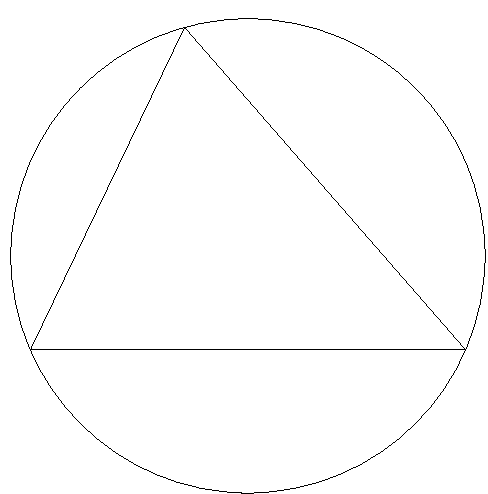
\includegraphics{./Non-isosceles.pdf}%
\end{picture}%
\setlength{\unitlength}{3947sp}%
%
\begingroup\makeatletter\ifx\SetFigFont\undefined%
\gdef\SetFigFont#1#2#3#4#5{%
  \reset@font\fontsize{#1}{#2pt}%
  \fontfamily{#3}\fontseries{#4}\fontshape{#5}%
  \selectfont}%
\fi\endgroup%
\begin{picture}(3888,3949)(2818,-3316)
\put(4152,486){\makebox(0,0)[lb]{\smash{{\SetFigFont{12}{14.4}{\familydefault}{\mddefault}{\updefault}{\color[rgb]{0,0,0}$B$}%
}}}}
\put(2833,-2262){\makebox(0,0)[lb]{\smash{{\SetFigFont{12}{14.4}{\familydefault}{\mddefault}{\updefault}{\color[rgb]{0,0,0}$A$}%
}}}}
\put(6603,-2232){\makebox(0,0)[lb]{\smash{{\SetFigFont{12}{14.4}{\familydefault}{\mddefault}{\updefault}{\color[rgb]{0,0,0}$C$}%
}}}}
\end{picture}%

\end{center}

\end{exer}
\clearpage

\noindent{\large \bf Exercises --- \thesection\ }

\begin{enumerate}
\item Prove that if the cube of an integer is odd, then that integer is odd.

\hint{The best hint for this problem is simply to write down the contrapositive statement. It is trivial to prove!}

\wbvfill

\item Prove that whenever a prime $p$ does not divide the square of an integer, 
it also doesn't divide the original integer. 
($p \nmid x^2 \; \implies \; p \nmid x$)

\hint{The contrapositive is $(p \divides x) \; \implies \; (p \divides x^2)$.}

\wbvfill

\workbookpagebreak

\item Prove (by contradiction) that there is no largest integer.

\hint{Well, if there was a largest integer -- let's call it $L$ (for largest) -- then isn't $L+1$ an integer, and isn't it bigger?  That's the main idea.  A more formal proof might look like this:

\begin{proof} 
Suppose (by way of contradiction) that there is a largest integer $L$.   Then $L \in \Integers$ and $\forall z \in \Integers, L \geq z$.
Consider the quantity $L+1$.  Clearly $L+1$ is an integer (because it is the sum of two integers) and also
$L+1 > L$.   This is a contradiction so the original supposition is false.   Hence there is no largest integer.
\end{proof}
}

\wbvfill

\item Prove (by contradiction) that there is no smallest positive real number.

\hint{Assume there was a smallest positive real number -- might as well call it $s$ (for smallest) -- what can we do to produce an even smaller number? (But be careful that it needs to remain positive -- for instance $s-1$ won't work.)}

\wbvfill

\workbookpagebreak

\item Prove (by contradiction) that the sum of a rational and an irrational 
number is irrational.

\hint{Suppose that x is rational and y is irrational and their sum (let's call it z) is also rational. Do some algebra to solve for y, and you will see that y (which is, by presumption, irrational) is also the difference of two rational numbers (and hence, rational -- a contradiction.)
}

\wbvfill

%\workbookpagebreak

\item Prove (by contraposition) that for all integers $x$ and $y$, if $x+y$ is odd, then $x\neq y$.

\hint{Well, the problem says to do this by contraposition, so let's write down the contrapositive:

\[ \forall x, y \in \Integers, \; x=y \, \implies \, x+y \; \mbox{is even}. \]

But proving that is obvious!
}

\wbvfill

\workbookpagebreak

\item Prove (by contraposition) that for all real numbers $a$ and $b$, if $ab$ is irrational, then $a$
is irrational or $b$ is irrational.

\hint{The contrapositive would be:

\[ \forall a,b \in \Reals, \; (a \in \Rationals \land b \in \Rationals) \, \implies ab \in \Rationals. \]

Wow! Haven't we proved that before?}

\wbvfill


%\workbookpagebreak

\item A \index{Pythagorean triple}\emph{Pythagorean triple} is a set of three
natural numbers, $a$, $b$ and $c$, such that $a^2 + b^2 = c^2$.  Prove that, in a
Pythagorean triple, at least one of $a$ and $b$ is even.  Use either a proof by
contradiction or a proof by contraposition.

\hint{If both $a$ and $b$ are odd then their squares will be 1 mod 4 -- so the sum of their squares
will be 2 mod 4.  But $c^2$ can only be 0 or 1 mod 4, which gives us a contradiction.}

\wbvfill

\workbookpagebreak

\item Suppose you have 2 pairs of positive real numbers whose products are 1.  That is, you have $(a,b)$ and $(c,d)$ in $\Reals^2$ satisfying $ab=cd=1$.  Prove that
$a < c$ implies that $b > d$.

 \hint{
 \begin{proof}
 Suppose by way of contradiction that $a,b,c,d \in \Reals$ satisfy $ab=cd=1$ and that $a<c$ and $b \leq d$.
 By multiplying the inequalities we get that $ab < cd$ which contradicts the assumption that both products
 are equal to 1 (and so must be equal to one another).
 \end{proof} 
  } 
  
  \wbvfill
  
  \workbookpagebreak
  
\end{enumerate}


\newpage

\section{Disproofs}
\label{sec:disproofs}

The idea of a ``disproof'' is really just semantics -- in order to
disprove a statement we need to \emph{prove} its negation.  

So far we've been discussing proofs quite a bit, but have paid
very little attention to a really huge issue.  If the statements
we are attempting to prove are false, no proof is ever going to
be possible.  Really, a prerequisite to developing a facility with
proofs is developing a good ``lie detector.''   We need to be able 
to guess, or quickly ascertain, whether a statement is true or false.
If we are given a universally quantified statement the first thing to
do is try it out for some random elements of the universe we're working
in.  If we happen across a value that satisfies the statement's hypotheses
but doesn't satisfy the conclusion, we've found what is known as a 
\index{counterexample}\emph{counterexample}.  

Consider the following statement about integers and divisibility:

\begin{conj} \label{conj:prim}
\[ \forall a,b,c \in \Integers, \; a \divides bc \; \implies \; a \divides b \,
\lor \, a \divides c. \]
\end{conj}

This is phrased as a UCS, so the hypothesis is clear, we're looking 
for three integers so that the first divides the product of the other
two. In the following table we have collected several values for
$a$, $b$ and $c$ such that $a \divides bc$.

\begin{center}
\begin{tabular}{c|c|c|c}
$a$ & $b$ & $c$ & $ a \divides b \, \lor \, a \divides c $ ? \\ \hline
2 & 7 & 6 & yes \\  
2 & 4 & 5 & yes \\  
3 & 12 & 11 & yes \\
3 & 5 & 15 & yes \\
5 & 4 & 15 & yes \\
5 & 10 & 3 & yes \\
7 & 2 & 14 & yes \\
\end{tabular}
\end{center}

\begin{exer} 
As noted in Section~\ref{sec:def} the statement above is related to
whether or not $a$ is prime.  Note that in the table, only prime
values of $a$ appear.  This is a rather broad hint.  Find a 
counterexample to Conjecture~\ref{conj:prim}.
\end{exer}

There can be times when the search for a counterexample starts to feel
really futile.  Would you think it likely that a statement about
natural numbers could be true for (more than) the first 50 numbers
a yet still be false?  

\begin{conj}
\label{conj:prim2}
\[ \forall n \in \Integers^+ \; n^2 - 79n + 1601 \, \mbox{is prime.} \]
\end{conj}

\begin{exer}
Find a counterexample to Conjecture~\ref{conj:prim2}
\end{exer}

Hidden within Euclid's proof of the infinitude of the primes is
a sequence.  Recall that in the proof we deduced a contradiction
by considering the number $N$ defined by 

\[  N = 1 + \prod_{k=1}^n p_k. \]

Define a sequence by

\[  N_n  = 1 + \prod_{k=1}^n p_k, \]

where $\{p_1, p_2, \ldots , p_n\}$ are the actual first $n$ primes.
The first several values of this sequence are:

\rule{72pt}{0pt} \begin{tabular}{c|c}
 $n$ & $N_n$ \\ \hline
 $1$ & $1+(2) = 3$ \\
 $2$ & $1+(2\cdot 3) = 7$\\
 $3$ & $1+(2\cdot 3\cdot 5) = 31$\\
 $4$ & $1+(2\cdot 3\cdot 5\cdot 7) = 211$\\
 $5$ & $1+(2\cdot 3\cdot 5\cdot 7\cdot 11) = 2311$\\
$\vdots$ & $\vdots$ \\
\end{tabular}

Now, in the proof, we deduced a contradiction by noting that $N_n$ is
much larger than $p_n$, so if $p_n$ is the largest prime it follows that
$N_n$ can't be prime -- but what really appears to be the case (just look 
at that table!) is that $N_n$ actually \emph{is} prime for all $n$. 

\begin{exer}
Find a counterexample to the conjecture that $1+\prod_{k=1}^n p_k$
is itself always a prime.
\end{exer}


\clearpage

\noindent{\large \bf Exercises --- \thesection\ }

\begin{enumerate}
\item Find a polynomial that assumes only prime values for
a reasonably large range of inputs.

\hint{It sort of depends on what is meant by ``a reasonably large range of inputs.''  For example the polynomial $p(x) = 2x+1$ gives primes three times in a row (at $x=1,2$ and $3$).  See if you can do better than that.
}
\item Find a counterexample to \ifthenelse{\boolean{InTextBook}}{Conjecture~\ref{conj:prim}}{the conjecture that $\forall a,b,c \in \Integers, a \divides bc \; \implies \; a \divides b \, \lor \, a \divides c$} using only powers of 2.

\hint{The intent of the problem is that you find three numbers, $a$, $b$ and $c$, that are all powers 
of $2$ and such that $a$ divides the product $bc$, but neither of the factors separately. For instance, 
if you pick $a=16$, then you would need to choose $b$ and $c$ so that $16$ doesn't divide evenly 
into them (they would need to be less than $16$\ldots) but so that their product {\em is} divisible by $16$.
}

\item The alternating sum of factorials provides an interesting
example of a sequence of integers.
\begin{center}
\[ 1! = 1 \]
\[ 2! - 1! = 1\]
\[ 3! - 2! + 1! = 5 \]
\[ 4! - 3! + 2! - 1! = 19 \]
et cetera
\end{center}

\noindent Are they all prime?  (After the first two 1's.)

\hint{

Here's some Sage code that would test this conjecture:

{\tt 
n=1\newline
for i in [2..8]:\newline
    n = factorial(i) - n\newline
    show(factor(n))\newline
}

Of course it turns out that going out to $8$ isn't quite far enough\ldots

}


\item It has been conjectured that whenever $p$ is prime, $2^p - 1$ is
also prime.  Find a minimal counterexample.

\hint{I would definitely seek help at your friendly neighborhood CAS.  In Sage 
you can loop over the first several prime numbers using the following syntax.

{\tt for p in [2,3,5,7,11,13]:}

\noindent If you want to automate that somewhat, there is a Sage function that returns a list
of all the primes in some range.  So the following does the same thing.

{\tt for p in primes(2,13):}


}
\item True or false:  The sum of any two irrational numbers is irrational.
Prove your answer.

\hint{This statement and the next are negations of one another.  Your answers should reflect that.}

\item True of false:  There are two irrational numbers whose sum is rational.
Prove your answer.

\hint{If a number is irrational, isn't its negative also irrational?  That's actually a pretty huge hint.}

\item True or false: The product of any two irrational numbers is irrational.
Prove your answer.

\hint{This one and the next are negations too. Aren't they?}

\item True or false: There are two irrational numbers whose product is rational.
Prove your answer.

\hint{The two numbers {\em could} be equal couldn't they?}

\item True or false:  Whenever an integer $n$ is a divisor of the square of an integer, $m^2$, it follows that $n$ is a divisor of $m$ as well.
(In symbols, $\forall n \in \Integers, \forall m \in \Integers, n \mid m^2 \; \implies \; n \mid m$.)
Prove your answer.

\hint{Hint: List all of the divisors of $36 = (2\cdot 3)^2$.  See if any of them are bigger than $6$.}

\item In an exercise in Section~\ref{sec:more} we proved that the quadratic 
equation $ax^2 + bx + c = 0$ has two solutions if $ac < 0$.  Find a counterexample which shows that this implication cannot be replaced with a biconditional.  

\hint{We'd want $ac$ to be positive (so $a$ and $c$ have the same sign) but nevertheless have $b^2-4ac > 0$.  It seems that if we make $b$ sufficiently large that could happen.}


\end{enumerate}



\newpage
\section[By cases and By exhaustion]{Even more direct proofs: By cases and By exhaustion}
\label{sec:cases}

\index{proof by exhaustion}
Proof by exhaustion is the least attractive proof method from 
an aesthetic perspective.  An exhaustive proof consists of literally
(and exhaustively) checking every element of the universe to see
if the given statement is true for it.  Usually, of course, this is
impossible because the universe of discourse is infinite; but when the
universe of discourse is finite, one certainly can't argue the validity
of an exhaustive proof.  

In the last few decades the introduction of powerful computational
assistance for mathematicians has lead to a funny situation.  There
is a growing list of important results that have been ``proved'' by
exhaustion using a computer.  Important examples of this phenomenon
are the non-existence of a 
\index{projective plane of order 10}
projective plane of order 10\cite{lam} and the 
only known value of a 
\index{Ramsey number}Ramsey number for hypergraphs\cite{radz}. 

\index{proof by cases}
Proof by cases is subtly different from exhaustive proof -- for one 
thing a valid proof by cases can be used in an infinite universe.  
In a proof by cases one has to divide the universe of discourse into
a finite number of sets\footnote{It is necessary to provide an argument that 
this list of cases is complete!  I.e. that every element of the universe
falls into one of the cases.} and then provide a separate proof for each
of the cases.  A great many statements about the integers can be proved
using the division of integers into even and odd.  Another set of 
cases that is used frequently is the finite number of possible remainders
obtained when dividing by an integer $d$.  (Note that even and odd correspond
to the remainders $0$ and $1$ obtained after division by $2$.)    
  
A very famous instance of proof by cases is the computer-assisted proof
of the 
\index{four color theorem}
four color theorem.  The four color theorem is a result known to
map makers for quite some time that says that 4 colors are always sufficient
to color the nations on a map in such a way that countries sharing a boundary
are always colored differently.  Figure~\ref{fig:Lux_map} shows one instance
of an arrangement of nations that requires at least four different colors, 
the theorem says that four colors are \emph{always} enough.  It should be noted
that real cartographers usually reserve a fifth color for oceans (and other 
water) and that it is possible to conceive of a map requiring five colors if 
one allows the nations to be non-contiguous.   In 1977, 
\index{Appel, Kenneth} Kenneth Appel and 
\index{Haken, Wolfgang}Wolfgang Haken proved the four color
theorem by reducing the infinitude of possibilities to 
1,936 separate cases and analyzing each of these with a computer.  
The inelegance of a proof by cases is probably proportional to some power of
the number of cases, but in any case, this proof is generally considered 
somewhat inelegant.  Ever since the proof was announced there has been an
ongoing effort to reduce the number of cases (currently the record is 633
cases -- still far too many to be checked through without a computer) or to
find a proof that does not rely on cases.  For a  good introductory article on
the four color theorem see\cite{wiki-4color}. 

\begin{figure}[!hbtp] 
\begin{center}
\begin{picture}(0,0)%
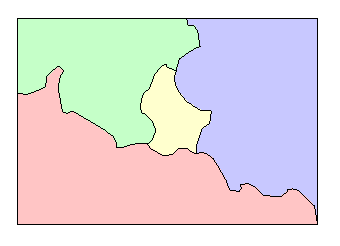
\includegraphics{figures/Luxembourg.pdf}%
\end{picture}%
\setlength{\unitlength}{3947sp}%
%
\begingroup\makeatletter\ifx\SetFigFont\undefined%
\gdef\SetFigFont#1#2#3#4#5{%
  \reset@font\fontsize{#1}{#2pt}%
  \fontfamily{#3}\fontseries{#4}\fontshape{#5}%
  \selectfont}%
\fi\endgroup%
\begin{picture}(2702,1952)(225,-1412)
\end{picture}%

\end{center}
\caption[A four-color map.]{The nations surrounding %
\index{Luxembourg} Luxembourg show %
that sometimes 4 colors are required in cartography.}
\label{fig:Lux_map}
\end{figure}

Most exhaustive proofs of statements that aren't trivial tend to either be (literally) too exhausting or to seem rather contrived.  One example of a situation
in which an exhaustive proof of some statement exists is when the statement
is thought to be universally true but no general proof is known -- yet the
statement has been checked for a large number of cases.  
\index{Goldbach's conjecture}Goldbach's conjecture
is one such statement.  
\index{Goldbach, Christian}Christian Goldbach~\cite{wiki-goldbach} 
was a mathematician born
in \index{K\"{o}nigsberg}K\"{o}nigsberg Prussia, 
who, curiously, did \emph{not} make the
conjecture\footnote{This conjecture was %
discussed previously in the exercises of Section~\ref{sec:def}} which bears
his name.  In a letter to 
\index{Euler, Leonhard}Leonard Euler, Goldbach conjectured that every
odd number greater than 5 could be expressed as the sum of three primes (nowadays this is known as the 
\index{weak Goldbach conjecture} weak Goldbach conjecture).  Euler apparently liked the 
problem and replied to Goldbach stating what is now known as Goldbach's 
conjecture: Every even number greater than 2 can be expressed as the sum of
two primes.  This statement has been lying around since 1742, and a great
many of the world's best mathematicians have made their attempts at proving it
-- to no avail! (Well, actually a lot of progress has been made but the result
still hasn't been proved.)  It's easy to verify the Goldbach conjecture for
relatively small even numbers, so what \emph{has} been done is/are proofs by
exhaustion of Goldbach's conjecture restricted to finite universes. 
As of this writing, the conjecture has been verified to be true of
all even numbers less than $2 \times 10^{17}$.      
 
Whenever an exhaustive proof, or a proof by cases exists for some statement
it is generally felt that a direct proof would be more esthetically pleasing.
If you are in a situation that doesn't admit such a direct proof, you should
at least seek a proof by cases using the minimum possible number of cases.
For example, consider the following theorem and proof.

\begin{thm} $\forall n \in \Integers \; n^2 \;$ is of the form $4k$ or 
$4k+1$ for some $k \in \Integers$.
\end{thm}

\begin{proof}
We will consider the four cases determined by the four
possible residues mod 4.

\begin{itemize}
\item[case i)] If $n \equiv 0 \pmod{4}$ then there is an integer $m$
such that $n = 4m$.  It follows that $n^2 = (4m)^2 = 16m^2$ is of the 
form $4k$ where $k$ is $4m^2$.

\item[case ii)] If $n \equiv 1 \pmod{4}$ then there is an integer $m$
such that $n = 4m+1$.  It follows that $n^2 = (4m+1)^2 = 16m^2 + 8m + 1$ 
is of the form $4k+1$ where $k$ is $4m^2+2m$.

\item[case iii)] If $n \equiv 2 \pmod{4}$ then there is an integer $m$
such that $n = 4m+2$.  It follows that $n^2 = (4m+2)^2 = 16m^2 + 16m + 4$ 
is of the form $4k$ where $k$ is $4m^2+4m+1$.

\item[case iv)] If $n \equiv 3 \pmod{4}$ then there is an integer $m$
such that $n = 4m+3$.  It follows that $n^2 = (4m+3)^2 = 16m^2 + 24m + 9$ 
is of the form $4k+1$ where $k$ is $4m^2+6m+2$.
\end{itemize}

Since these four cases exhaust the possibilities and since the desired
result holds in each case, our proof is complete.

\end{proof} 

While the proof just stated is certainly valid, the argument is inelegant
since a smaller number of cases would suffice.

\begin{exer}
The previous theorem can be proved using just two cases.  Do so.
\end{exer}

We'll close this section by asking you to determine an exhaustive proof where 
the complexity of the argument is challenging but not \emph{too} impossible.

\index{graph pebbling} Graph pebbling is an interesting concept originated 
by the famous combinatorialist \index{Chung, Fan} Fan Chung.  A ``graph'' 
(as the term is used here) is a collection
of places or locations which are known as ``nodes,'' some of which 
are joined by paths or connections which are known as ``edges.'' 
Graphs have been studied by mathematicians for about 400 years, and 
many interesting problems can be put in this setting.  Graph pebbling
is a crude version of a broader problem in resource management -- often
a resource actually gets used in the process of transporting it.  Think of
the big tanker trucks that are used to transport gasoline.  What do they
run on?  Well, actually they probably burn diesel --- but the point is
that in order to move the fuel around we have to consume some of it.
Graph pebbling takes this to an extreme: in order to move one pebble
we must consume one pebble.  

Imagine that a bunch of pebbles are randomly
distributed on the nodes of a graph, and that we are allowed to do 
\emph{graph pebbling moves} -- we remove two pebbles from some node
and place a single pebble on a node that is connected to it.
See Figure~\ref{fig:pebbling_move}.

\begin{figure}[!hbtp] 
\begin{center}
\begin{picture}(0,0)%
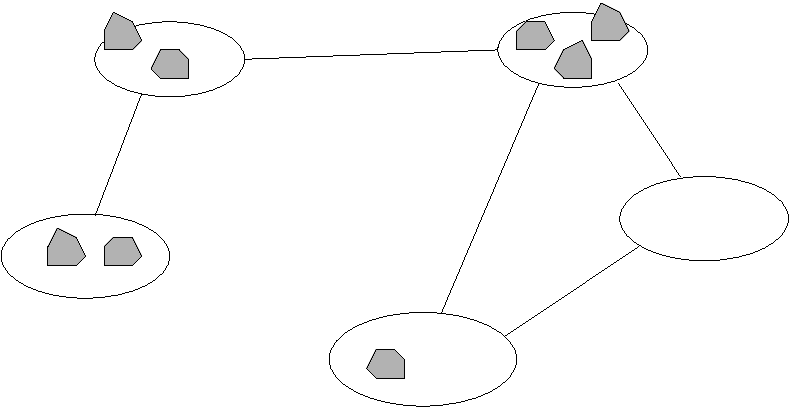
\includegraphics{figures/pebbling.pdf}%
\end{picture}%
\setlength{\unitlength}{3947sp}%
%
\begingroup\makeatletter\ifx\SetFigFont\undefined%
\gdef\SetFigFont#1#2#3#4#5{%
  \reset@font\fontsize{#1}{#2pt}%
  \fontfamily{#3}\fontseries{#4}\fontshape{#5}%
  \selectfont}%
\fi\endgroup%
\begin{picture}(6326,3252)(1268,-2776)
\put(5401,-2761){\makebox(0,0)[lb]{\smash{{\SetFigFont{12}{14.4}{\familydefault}{\mddefault}{\updefault}{\color[rgb]{0,0,0}E}%
}}}}
\put(2701,-1711){\makebox(0,0)[lb]{\smash{{\SetFigFont{12}{14.4}{\familydefault}{\mddefault}{\updefault}{\color[rgb]{0,0,0}A}%
}}}}
\put(3151,-361){\makebox(0,0)[lb]{\smash{{\SetFigFont{12}{14.4}{\familydefault}{\mddefault}{\updefault}{\color[rgb]{0,0,0}B}%
}}}}
\put(6526,-211){\makebox(0,0)[lb]{\smash{{\SetFigFont{12}{14.4}{\familydefault}{\mddefault}{\updefault}{\color[rgb]{0,0,0}C}%
}}}}
\put(7426,-1711){\makebox(0,0)[lb]{\smash{{\SetFigFont{12}{14.4}{\familydefault}{\mddefault}{\updefault}{\color[rgb]{0,0,0}D}%
}}}}
\end{picture}%

\end{center}
\caption[Graph pebbling.]{In graph pebbling problems a collection of pebbles
are distributed on the nodes of a graph.  There is no significance to the 
particular graph that is shown here, or to the arrangement of pebbles -- 
we are just giving an example.}
\label{fig:pebbling}
\end{figure}

\begin{figure}[!hbtp] 
\begin{center}
\begin{picture}(0,0)%
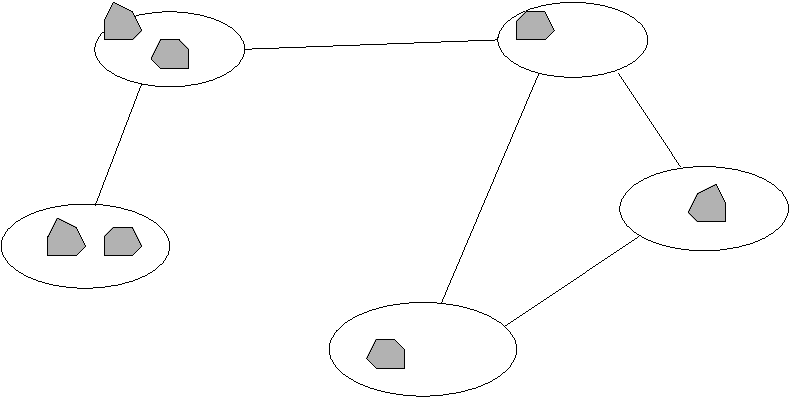
\includegraphics{./pebbling_move.pdf}%
\end{picture}%
\setlength{\unitlength}{3947sp}%
%
\begingroup\makeatletter\ifx\SetFigFont\undefined%
\gdef\SetFigFont#1#2#3#4#5{%
  \reset@font\fontsize{#1}{#2pt}%
  \fontfamily{#3}\fontseries{#4}\fontshape{#5}%
  \selectfont}%
\fi\endgroup%
\begin{picture}(6326,3177)(1268,-2776)
\put(5401,-2761){\makebox(0,0)[lb]{\smash{{\SetFigFont{12}{14.4}{\familydefault}{\mddefault}{\updefault}{\color[rgb]{0,0,0}E}%
}}}}
\put(2701,-1711){\makebox(0,0)[lb]{\smash{{\SetFigFont{12}{14.4}{\familydefault}{\mddefault}{\updefault}{\color[rgb]{0,0,0}A}%
}}}}
\put(3151,-361){\makebox(0,0)[lb]{\smash{{\SetFigFont{12}{14.4}{\familydefault}{\mddefault}{\updefault}{\color[rgb]{0,0,0}B}%
}}}}
\put(6526,-211){\makebox(0,0)[lb]{\smash{{\SetFigFont{12}{14.4}{\familydefault}{\mddefault}{\updefault}{\color[rgb]{0,0,0}C}%
}}}}
\put(7426,-1711){\makebox(0,0)[lb]{\smash{{\SetFigFont{12}{14.4}{\familydefault}{\mddefault}{\updefault}{\color[rgb]{0,0,0}D}%
}}}}
\end{picture}%

\end{center}
\caption[Graph pebbling move.]{A graph pebbling move takes two pebbles off
of a node and puts one of them on an adjacent node (the other is discarded).
Notice how node C, which formerly held 3 pebbles, now has only 1 and that 
a pebble is now present on node D where previously there was none.}
\label{fig:pebbling_move}
\end{figure}

For any particular graph, we can ask for its \emph{pebbling number}, $\rho$.  
This is the smallest number so that if $\rho$ pebbles are distributed {\em in any way whatsoever} on the nodes of the graph, it will be possible to use 
pebbling moves so as to get a pebble to any node. 

For example, consider the triangle graph -- three nodes which are all 
mutually connected.  The pebbling number of this graph is 3.  If we
start with one pebble on each node we are already done; if there is a 
node that has two pebbles on it, we can use a pebbling move to reach
either of the other two nodes.

\begin{exer} 
There is a graph $C_5$ which consists of 5 nodes connected in a circular
fashion.  Determine its pebbling number.  Prove your answer exhaustively.

Hint: the pebbling number must be greater than 4 because if one pebble is
placed on each of 4 nodes the configuration is unmovable (we need to 
have two pebbles on a node in order to be able to make a pebbling move
at all) and so the 5th node can never be reached.
\end{exer}
 
\clearpage

\noindent{\large \bf Exercises --- \thesection\ }

\begin{enumerate}
\item Prove that if $n$ is an odd number then $n^4 \pmod{16} = 1$.

\hint{

While one could perform fairly complicated arithmetic, expanding expression like
$(16k+13)^4$ and then regrouping to put it in the form $16q+1$ (and one would need 
to do that work for each of the odd remainders modulo $16$),  that would be missing out
on the true power of modular notation.  In a ``$\pmod{16}$'' calculation one can simply ignore
summands like $16k$ because they are $0 \pmod{16}$.  Thus, for example,

  \[ (16k+7)^4 \pmod{16} \; = \; 7^4 \pmod{16} \; = \; 2401 \pmod{16}  \; = \; 1. \]
  
So, essentially one just needs to compute the $4$th powers of $1, 3, 5, 7, 9, 11, 13$  and $15$, and
then reduce them modulo 16.  An even greater economy is possible if one notes that (modulo 16) many
of those cases are negatives of one another -- so their $4$th powers are equal.
}

\wbvfill
     
\item Prove that every prime number other than 2 and 3 has the form
$6q+1$ or $6q+5$ for some integer $q$.  (Hint: this problem involves
thinking about cases as well as contrapositives.)

\hint{It is probably obvious that the "cases" will be the possible remainders mod 6. Numbers of the form 6q+0 will be multiples of 6, so clearly not prime. The other forms that need to be eliminated are 6q+2, 6q+3, and 6q+4.
}

\wbvfill

\workbookpagebreak

\item Show that the sum of any three consecutive integers is divisible
by 3.

\hint{Write the sum as $n + (n+1) + (n+2)$.}

\wbvfill

\item There is a graph known as $K_4$ that has $4$ nodes and there is an edge between every pair of nodes.
The pebbling number of $K_4$ has to be at least $4$ since it would be possible to put one pebble on each of
$3$ nodes and not be able to reach the remaining node using pebbling moves.  Show that the pebbling number of $K_4$ is actually $4$.

\hint{If there are two pebbles on any node we will be able to reach all the other nodes using pebbling moves
(since every pair of nodes is connected).}

\wbvfill

\workbookpagebreak

\item Find the pebbling number of a graph whose nodes are the corners and 
whose edges are the, uhmm, edges of a cube.

\hint{It should be clear that the pebbling number is at least $8$ -- $7$ pebbles could be distributed, 
one to a node, and the $8$th node would be unreachable.  It will be easier to play around with this if
you figure out how to draw the cube graph ``flattened-out'' in the plane.}

\wbvfill

\item A \index{vampire number}\emph{vampire number} is a $2n$ digit number $v$ that factors as $v=xy$
where $x$ and $y$ are $n$ digit numbers and the digits of $v$ are the 
union of the digits in $x$ and $y$ in some order.  The numbers $x$ and $y$
are known as the ``fangs'' of $v$.  To eliminate trivial
cases, pairs of trailing zeros are disallowed.  

Show that there are no 2-digit vampire numbers.

Show that there are seven 4-digit vampire numbers.

\hint{The 2-digit challenge is do-able by hand (just barely).  The $4$ digit question certainly requires 
some computer assistance!}

\wbvfill

\workbookpagebreak

\item Lagrange's theorem on representation of integers as sums of squares
says that every positive integer can be expressed as the sum of at most 
$4$ squares.  For example, $79 = 7^2 + 5^2 + 2^2 + 1^2$.  Show (exhaustively) 
that $15$ can not be represented using fewer than $4$ squares.

\hint{Note that $15 = 3^2 + 2^2 + 1^2 + 1^2$.  Also, if $15$ were expressible as a sum of fewer than $4$ squares, the squares involved would be $1$, $4$ and $9$.  It's really not that hard to try all the possibilities.}

\wbvfill

\item Show that there are exactly $15$ numbers $x$ in the range $1 \leq x \leq 100$ that can't be represented using fewer than $4$ squares.



\hint{The following Sage code generates all the numbers up to $100$ that {\em can} be written
as the sum of at most $3$ squares.

{\tt
var('x y z') \newline
a=[s$\caret$2 for s in [1..10]]  \newline
b=[s$\caret$2 for s in [0..10]]  \newline
s = []  \newline
for x in a:  \newline
\tab for y in b:  \newline
\tab \tab for z in b:  \newline
\tab \tab \tab s = union(s,[x+y+z])  \newline
s = Set(s)  \newline
H=Set([1..100]) \newline
show(H.intersection(s))  \newline
}
}

\wbvfill

\workbookpagebreak

\item The \index{trichotomy property}\emph{trichotomy property} of the real 
numbers simply states that every real number is either positive or negative 
or zero.  Trichotomy can be used to prove many statements by looking at the
three cases that it guarantees.  Develop a proof (by cases) that the square of
any real number is non-negative.

\hint{By trichotomy, x is either zero, negative, or positive. If x is zero, its square is zero. If x is negative, its square is positive. If x is positive, its square is also positive.}

\wbvfill

\item Consider the game called ``binary determinant tic-tac-toe''\footnote{ %
This question was problem A4 in the 63rd annual %
\index{William Lowell Putnam Mathematics Competition} %
William Lowell Putnam Mathematics Competition (2002).  %
There are three collections of questions %
and answers  from previous Putnam exams available from the MAA % 
\cite{putnam1,putnam2,putnam3}% 
}
which is played by two players who alternately fill in the entries of a 
$3 \times 3$ array.  Player One goes first, placing 1's in the array and 
player Zero goes second, placing 0's.  Player One's goal is that the 
final array have determinant 1, and player Zero's goal is that the 
determinant be 0.  The determinant calculations are carried out mod 2.

Show that player Zero can always win a game of binary determinant tic-tac-toe
by the method of exhaustion.

\hint{If you know something about determinants it would help here.  The determinant will be
0 if there are two identical rows (or columns) in the finished array.  Also, if there is a row or column
that is all zeros, player Zero wins too.  Also, cyclically permuting either rows or columns has no effect
on the determinant of a binary array.  This means we lose no generality in assuming player One's
first move goes (say) in the upper-left corner.}

\wbvfill

\workbookpagebreak

\rule{0pt}{0pt}

\workbookpagebreak

\end{enumerate}



\newpage

\section[Existential statements]{Proofs and disproofs of existential statements}
\label{sec:exist}

From a certain point of view, there is no need for the current section.
If we are proving an existential statement we are \emph{disproving} some
universal statement. (Which has already been discussed.)  Similarly,
if we are trying to disprove an existential statement, then we are
actually \emph{proving} a related universal statement.  Nevertheless,
sometimes the way a theorem is stated emphasizes the existence question
over the corresponding universal -- and so people talk about proving
and disproving existential statements as a separate issue from 
universal statements.

Proofs of existential questions come in two basic varieties: constructive
and non-constructive.  Constructive proofs are conceptually the easier
of the two -- you actually name an example that shows the existential
question is true.  For example:

\begin{thm}
There is an even prime.
\end{thm}

\begin{proof}
The number 2 is both even and prime. 
\end{proof} 

\begin{exer}
The Fibonacci numbers are defined by the initial values $F(0)=1$
and $F(1)=1$ and the recursive formula $F(n+1) = F(n)+F(n-1)$ (to
get the next number in the series you add the last and the penultimate).

\rule{72pt}{0pt} \begin{tabular}{c|c}
$n$ & $F(n)$ \\ \hline
0 & 1 \\
1 & 1 \\
2 & 2 \\
3 & 3 \\
4 & 5 \\
5 & 8 \\
$\vdots$ & $\vdots$\\
\end{tabular}
\medskip

Prove that there is a Fibonacci number that is a perfect square.
\end{exer}

A non-constructive existence proof is trickier.  One approach is to argue
by contradiction -- if the thing we're seeking doesn't exist that will
lead to an absurdity.  Another approach is to outline a search algorithm
for the desired item and provide an argument as to why it cannot fail!

A particularly neat approach is to argue using dilemma.
This is my favorite non-constructive existential theorem/proof.

\begin{thm}
There are irrational numbers $\alpha$ and $\beta$ such that $\alpha^\beta$
is rational.
\end{thm}

\begin{proof}
If $\sqrt{2}^{\sqrt{2}}$ is rational then we are done.
(Let $ \alpha = \beta = \sqrt{2}$.)  Otherwise, let 
$\alpha = \sqrt{2}^{\sqrt{2}}$ and $\beta = \sqrt{2}$.  The result
follows because $\left(\sqrt{2}^{\sqrt{2}}\right)^{\sqrt{2}} = \sqrt{2}^{(\sqrt{2}\sqrt{2})} 
= \sqrt{2}^2 = 2$, which is clearly rational.

\end{proof} 

Many existential proofs involve a property of the natural numbers
known as the \index{well-ordering principle}well-ordering principle.  The well-ordering principle is 
sometimes abbreviated WOP.  If a set has WOP it doesn't mean that the 
set is ordered in a particularly good way, but rather that its subsets
are like wells -- the kind one hoists water out of with a bucket on a rope.
You needn't be concerned with WOP in general at this point, but notice
that the subsets of the natural numbers have a particularly nice property
 -- any non-empty set of natural numbers must have a least element (much like
every water well has a bottom).

Because the natural numbers have the well-ordering principle 
we can prove that there is a least 
natural number with property X by simply finding \emph{any} natural
number with property X -- by doing that we've shown that the set of
natural numbers with property X is non-empty and that's the only
hypothesis the WOP needs.  

For example, in the exercises in Section~\ref{sec:cases} we 
introduced vampire numbers. A \index{vampire number} \emph{vampire number} 
is a 
$2n$ digit number $v$ that factors as $v=xy$
where $x$ and $y$ are $n$ digit numbers and the digits of $v$ are the 
union of the digits in $x$ and $y$ in some order.  The numbers $x$ and $y$
are known as the ``fangs'' of $v$.  To eliminate trivial
cases, pairs of trailing zeros are disallowed.  


\begin{thm}
There is a smallest 6-digit vampire number.
\end{thm}

\begin{proof}
The number $125460$ is a vampire number (in fact this is the smallest
example of a vampire number with two sets of fangs: 
$125460 = 204\cdot 615 = 246\cdot 510$).  Since the set of 6-digit vampire
numbers is non-empty, the well-ordering principle of the natural numbers
allows us to deduce that there is a smallest 6-digit vampire number.
\end{proof} 
 
This is quite an interesting situation in that we know there is a smallest
6-digit vampire number without having any idea what it is!

\begin{exer}
Show that $102510$ is the smallest 6-digit vampire number.
\end{exer}

There are quite a few occasions when we need to prove statements
involving the \index{unique existence} unique existence quantifier 
($\exists !$).  In
such instances we need to do just a little bit more work.  We
need to show existence -- either constructively or non-constructively --
and we also need to show uniqueness.  To give an example of 
a unique existence proof we'll return to a concept first
discussed in Section~\ref{sec:alg} and finish-up some business
that was glossed-over there.

Recall the Euclidean algorithm that was used to calculate the 
\index{greatest common divisor, gcd}greatest
common divisor of two integers $a$ and $b$ (which we denote $\gcd{a}{b}$).
There is a rather important question concerning algorithms known as
the ``halting problem.''  Does the program eventually halt, or does it get 
stuck in an infinite loop?  We know that the Euclidean algorithm halts
(and outputs the correct result) because we know the following
unique existence result.

\[ \forall a, b \in \Integers^+, \, \exists ! \, d \in \Integers^+ \; \mbox{such that} \, d=\gcd{a}{b} \]
  
Now, before we can prove this result, we'll need a precise definition
for $\gcd{a}{b}$.   Firstly, a gcd must be a \emph{common divisor} which
means it needs to divide both $a$ and $b$.  Secondly, among all the common 
divisors, it must be the \emph{largest}.  This second point is usually 
addressed
by requiring that every other common divisor divides the gcd. Finally we 
should note that a gcd is always positive, for whenever a number divides
another number so does its negative, and whichever of those two is positive
will clearly be the greater!  This allows us to extend the definition of
gcd to all integers, but things are conceptually easier if we 
keep our attention restricted to the positive integers. 

\begin{defi}
The \emph{greatest common divisor}, or gcd, of two positive 
integers $a$ and $b$
is a positive integer $d$ such that $d \divides a$ and $d \divides b$ and if $c$ is any
other positive integer such that $c \divides a$ and $c \divides b$ then $c \divides d$.
  
\[ \forall a,b,c,d \in \Integers^+ \; d=\gcd{a}{b} \; \iff \;
d \divides a \, \land \, d \divides b \, \land \, (c \divides a \, \land \, c \divides b  \implies c \divides d)\]
\end{defi}

Armed with this definition, let's return our attention to proving the
unique existence of the gcd.  The uniqueness part is easier so we'll
do that first.  We argue by contradiction.  Suppose that there were
two different numbers $d$ and $d'$ satisfying the definition of $\gcd{a}{b}$.
Put $d'$ in the place of $c$ in the definition to see that $d' \divides d$.
Similarly, we can deduce that $d \divides d'$ and if two numbers each divide 
into the other, they must be equal.  This is a contradiction since we
assumed $d$ and $d'$ were different.

For the existence part we'll need to define a set -- known as the 
\index{Z-module}$\Integers$-module generated by $a$ and $b$ -- that consists of all 
numbers of the form $xa+yb$ where $x$ and $y$ range over the integers.

\begin{figure}[!hbtp] 
\begin{center}
\begin{picture}(0,0)%
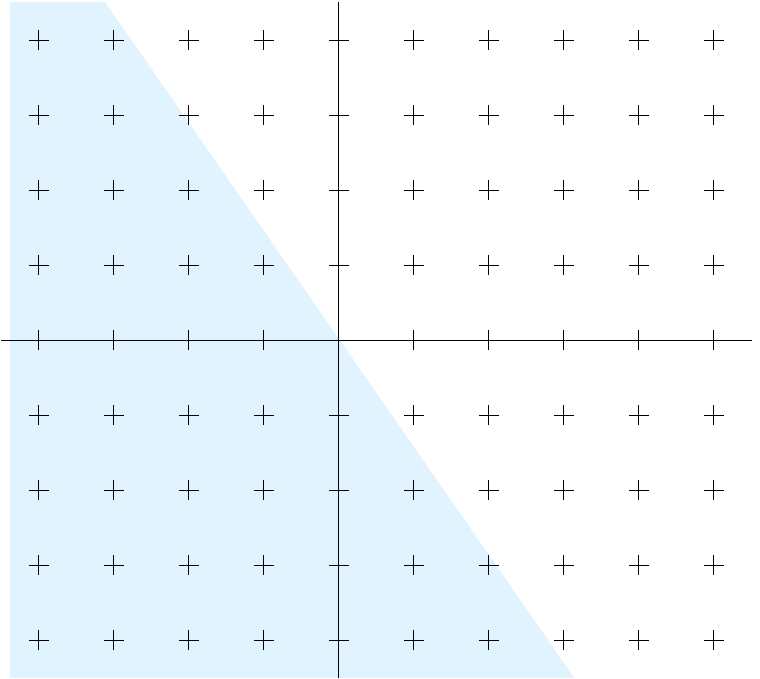
\includegraphics{figures/Z-module.pdf}%
\end{picture}%
\setlength{\unitlength}{3947sp}%
%
\begingroup\makeatletter\ifx\SetFigFont\undefined%
\gdef\SetFigFont#1#2#3#4#5{%
  \reset@font\fontsize{#1}{#2pt}%
  \fontfamily{#3}\fontseries{#4}\fontshape{#5}%
  \selectfont}%
\fi\endgroup%
\begin{picture}(6078,5424)(2089,-5473)
\put(4876,-2086){\makebox(0,0)[lb]{\smash{{\SetFigFont{12}{14.4}{\familydefault}{\mddefault}{\updefault}{\color[rgb]{0,0,0}15}%
}}}}
\put(5476,-2686){\makebox(0,0)[lb]{\smash{{\SetFigFont{12}{14.4}{\familydefault}{\mddefault}{\updefault}{\color[rgb]{0,0,0}21}%
}}}}
\put(5476,-2086){\makebox(0,0)[lb]{\smash{{\SetFigFont{12}{14.4}{\familydefault}{\mddefault}{\updefault}{\color[rgb]{0,0,0}36}%
}}}}
\put(6076,-2686){\makebox(0,0)[lb]{\smash{{\SetFigFont{12}{14.4}{\familydefault}{\mddefault}{\updefault}{\color[rgb]{0,0,0}42}%
}}}}
\put(6676,-2686){\makebox(0,0)[lb]{\smash{{\SetFigFont{12}{14.4}{\familydefault}{\mddefault}{\updefault}{\color[rgb]{0,0,0}63}%
}}}}
\put(7276,-2686){\makebox(0,0)[lb]{\smash{{\SetFigFont{12}{14.4}{\familydefault}{\mddefault}{\updefault}{\color[rgb]{0,0,0}84}%
}}}}
\put(7876,-2686){\makebox(0,0)[lb]{\smash{{\SetFigFont{12}{14.4}{\familydefault}{\mddefault}{\updefault}{\color[rgb]{0,0,0}105}%
}}}}
\put(4276,-2686){\makebox(0,0)[lb]{\smash{{\SetFigFont{12}{14.4}{\familydefault}{\mddefault}{\updefault}{\color[rgb]{0,0,0}-21}%
}}}}
\put(3676,-2686){\makebox(0,0)[lb]{\smash{{\SetFigFont{12}{14.4}{\familydefault}{\mddefault}{\updefault}{\color[rgb]{0,0,0}-42}%
}}}}
\put(3076,-2686){\makebox(0,0)[lb]{\smash{{\SetFigFont{12}{14.4}{\familydefault}{\mddefault}{\updefault}{\color[rgb]{0,0,0}-63}%
}}}}
\put(2476,-2686){\makebox(0,0)[lb]{\smash{{\SetFigFont{12}{14.4}{\familydefault}{\mddefault}{\updefault}{\color[rgb]{0,0,0}-84}%
}}}}
\put(4876,-3286){\makebox(0,0)[lb]{\smash{{\SetFigFont{12}{14.4}{\familydefault}{\mddefault}{\updefault}{\color[rgb]{0,0,0}-15}%
}}}}
\put(4876,-3886){\makebox(0,0)[lb]{\smash{{\SetFigFont{12}{14.4}{\familydefault}{\mddefault}{\updefault}{\color[rgb]{0,0,0}-30}%
}}}}
\put(4876,-4486){\makebox(0,0)[lb]{\smash{{\SetFigFont{12}{14.4}{\familydefault}{\mddefault}{\updefault}{\color[rgb]{0,0,0}-45}%
}}}}
\put(4876,-5086){\makebox(0,0)[lb]{\smash{{\SetFigFont{12}{14.4}{\familydefault}{\mddefault}{\updefault}{\color[rgb]{0,0,0}-60}%
}}}}
\put(4876,-1486){\makebox(0,0)[lb]{\smash{{\SetFigFont{12}{14.4}{\familydefault}{\mddefault}{\updefault}{\color[rgb]{0,0,0}30}%
}}}}
\put(4876,-886){\makebox(0,0)[lb]{\smash{{\SetFigFont{12}{14.4}{\familydefault}{\mddefault}{\updefault}{\color[rgb]{0,0,0}45}%
}}}}
\put(4876,-286){\makebox(0,0)[lb]{\smash{{\SetFigFont{12}{14.4}{\familydefault}{\mddefault}{\updefault}{\color[rgb]{0,0,0}60}%
}}}}
\put(5476,-1486){\makebox(0,0)[lb]{\smash{{\SetFigFont{12}{14.4}{\familydefault}{\mddefault}{\updefault}{\color[rgb]{0,0,0}51}%
}}}}
\put(5476,-886){\makebox(0,0)[lb]{\smash{{\SetFigFont{12}{14.4}{\familydefault}{\mddefault}{\updefault}{\color[rgb]{0,0,0}66}%
}}}}
\put(5476,-286){\makebox(0,0)[lb]{\smash{{\SetFigFont{12}{14.4}{\familydefault}{\mddefault}{\updefault}{\color[rgb]{0,0,0}81}%
}}}}
\put(4876,-2686){\makebox(0,0)[lb]{\smash{{\SetFigFont{12}{14.4}{\familydefault}{\mddefault}{\updefault}{\color[rgb]{0,0,0}0}%
}}}}
\put(4276,-3286){\makebox(0,0)[lb]{\smash{{\SetFigFont{12}{14.4}{\familydefault}{\mddefault}{\updefault}{\color[rgb]{0,0,0}-36}%
}}}}
\put(4276,-3886){\makebox(0,0)[lb]{\smash{{\SetFigFont{12}{14.4}{\familydefault}{\mddefault}{\updefault}{\color[rgb]{0,0,0}-51}%
}}}}
\put(4276,-4486){\makebox(0,0)[lb]{\smash{{\SetFigFont{12}{14.4}{\familydefault}{\mddefault}{\updefault}{\color[rgb]{0,0,0}-66}%
}}}}
\put(4276,-5086){\makebox(0,0)[lb]{\smash{{\SetFigFont{12}{14.4}{\familydefault}{\mddefault}{\updefault}{\color[rgb]{0,0,0}-81}%
}}}}
\put(6076,-2086){\makebox(0,0)[lb]{\smash{{\SetFigFont{12}{14.4}{\familydefault}{\mddefault}{\updefault}{\color[rgb]{0,0,0}57}%
}}}}
\put(6076,-1486){\makebox(0,0)[lb]{\smash{{\SetFigFont{12}{14.4}{\familydefault}{\mddefault}{\updefault}{\color[rgb]{0,0,0}72}%
}}}}
\put(6076,-886){\makebox(0,0)[lb]{\smash{{\SetFigFont{12}{14.4}{\familydefault}{\mddefault}{\updefault}{\color[rgb]{0,0,0}87}%
}}}}
\put(6076,-286){\makebox(0,0)[lb]{\smash{{\SetFigFont{12}{14.4}{\familydefault}{\mddefault}{\updefault}{\color[rgb]{0,0,0}102}%
}}}}
\put(6676,-2086){\makebox(0,0)[lb]{\smash{{\SetFigFont{12}{14.4}{\familydefault}{\mddefault}{\updefault}{\color[rgb]{0,0,0}78}%
}}}}
\put(6676,-1486){\makebox(0,0)[lb]{\smash{{\SetFigFont{12}{14.4}{\familydefault}{\mddefault}{\updefault}{\color[rgb]{0,0,0}93}%
}}}}
\put(6676,-886){\makebox(0,0)[lb]{\smash{{\SetFigFont{12}{14.4}{\familydefault}{\mddefault}{\updefault}{\color[rgb]{0,0,0}108}%
}}}}
\put(6676,-286){\makebox(0,0)[lb]{\smash{{\SetFigFont{12}{14.4}{\familydefault}{\mddefault}{\updefault}{\color[rgb]{0,0,0}123}%
}}}}
\put(7276,-2086){\makebox(0,0)[lb]{\smash{{\SetFigFont{12}{14.4}{\familydefault}{\mddefault}{\updefault}{\color[rgb]{0,0,0}99}%
}}}}
\put(7276,-1486){\makebox(0,0)[lb]{\smash{{\SetFigFont{12}{14.4}{\familydefault}{\mddefault}{\updefault}{\color[rgb]{0,0,0}114}%
}}}}
\put(7276,-886){\makebox(0,0)[lb]{\smash{{\SetFigFont{12}{14.4}{\familydefault}{\mddefault}{\updefault}{\color[rgb]{0,0,0}129}%
}}}}
\put(7276,-286){\makebox(0,0)[lb]{\smash{{\SetFigFont{12}{14.4}{\familydefault}{\mddefault}{\updefault}{\color[rgb]{0,0,0}144}%
}}}}
\put(7876,-2086){\makebox(0,0)[lb]{\smash{{\SetFigFont{12}{14.4}{\familydefault}{\mddefault}{\updefault}{\color[rgb]{0,0,0}120}%
}}}}
\put(7876,-1486){\makebox(0,0)[lb]{\smash{{\SetFigFont{12}{14.4}{\familydefault}{\mddefault}{\updefault}{\color[rgb]{0,0,0}135}%
}}}}
\put(7876,-886){\makebox(0,0)[lb]{\smash{{\SetFigFont{12}{14.4}{\familydefault}{\mddefault}{\updefault}{\color[rgb]{0,0,0}150}%
}}}}
\put(7876,-286){\makebox(0,0)[lb]{\smash{{\SetFigFont{12}{14.4}{\familydefault}{\mddefault}{\updefault}{\color[rgb]{0,0,0}165}%
}}}}
\put(5476,-3286){\makebox(0,0)[lb]{\smash{{\SetFigFont{12}{14.4}{\familydefault}{\mddefault}{\updefault}{\color[rgb]{0,0,0}6}%
}}}}
\put(6076,-3286){\makebox(0,0)[lb]{\smash{{\SetFigFont{12}{14.4}{\familydefault}{\mddefault}{\updefault}{\color[rgb]{0,0,0}27}%
}}}}
\put(6676,-3286){\makebox(0,0)[lb]{\smash{{\SetFigFont{12}{14.4}{\familydefault}{\mddefault}{\updefault}{\color[rgb]{0,0,0}48}%
}}}}
\put(7276,-3286){\makebox(0,0)[lb]{\smash{{\SetFigFont{12}{14.4}{\familydefault}{\mddefault}{\updefault}{\color[rgb]{0,0,0}69}%
}}}}
\put(7876,-3286){\makebox(0,0)[lb]{\smash{{\SetFigFont{12}{14.4}{\familydefault}{\mddefault}{\updefault}{\color[rgb]{0,0,0}90}%
}}}}
\put(5476,-3886){\makebox(0,0)[lb]{\smash{{\SetFigFont{12}{14.4}{\familydefault}{\mddefault}{\updefault}{\color[rgb]{0,0,0}-9}%
}}}}
\put(6076,-3886){\makebox(0,0)[lb]{\smash{{\SetFigFont{12}{14.4}{\familydefault}{\mddefault}{\updefault}{\color[rgb]{0,0,0}12}%
}}}}
\put(6676,-3886){\makebox(0,0)[lb]{\smash{{\SetFigFont{12}{14.4}{\familydefault}{\mddefault}{\updefault}{\color[rgb]{0,0,0}33}%
}}}}
\put(7276,-3886){\makebox(0,0)[lb]{\smash{{\SetFigFont{12}{14.4}{\familydefault}{\mddefault}{\updefault}{\color[rgb]{0,0,0}54}%
}}}}
\put(7876,-3886){\makebox(0,0)[lb]{\smash{{\SetFigFont{12}{14.4}{\familydefault}{\mddefault}{\updefault}{\color[rgb]{0,0,0}75}%
}}}}
\put(4276,-2086){\makebox(0,0)[lb]{\smash{{\SetFigFont{12}{14.4}{\familydefault}{\mddefault}{\updefault}{\color[rgb]{0,0,0}-6}%
}}}}
\put(3676,-2086){\makebox(0,0)[lb]{\smash{{\SetFigFont{12}{14.4}{\familydefault}{\mddefault}{\updefault}{\color[rgb]{0,0,0}-27}%
}}}}
\put(3076,-2086){\makebox(0,0)[lb]{\smash{{\SetFigFont{12}{14.4}{\familydefault}{\mddefault}{\updefault}{\color[rgb]{0,0,0}-48}%
}}}}
\put(4276,-1486){\makebox(0,0)[lb]{\smash{{\SetFigFont{12}{14.4}{\familydefault}{\mddefault}{\updefault}{\color[rgb]{0,0,0}9}%
}}}}
\put(3676,-1486){\makebox(0,0)[lb]{\smash{{\SetFigFont{12}{14.4}{\familydefault}{\mddefault}{\updefault}{\color[rgb]{0,0,0}-12}%
}}}}
\put(3076,-1486){\makebox(0,0)[lb]{\smash{{\SetFigFont{12}{14.4}{\familydefault}{\mddefault}{\updefault}{\color[rgb]{0,0,0}-33}%
}}}}
\put(4276,-886){\makebox(0,0)[lb]{\smash{{\SetFigFont{12}{14.4}{\familydefault}{\mddefault}{\updefault}{\color[rgb]{0,0,0}24}%
}}}}
\put(3676,-886){\makebox(0,0)[lb]{\smash{{\SetFigFont{12}{14.4}{\familydefault}{\mddefault}{\updefault}{\color[rgb]{0,0,0}3}%
}}}}
\put(2476,-1486){\makebox(0,0)[lb]{\smash{{\SetFigFont{12}{14.4}{\familydefault}{\mddefault}{\updefault}{\color[rgb]{0,0,0}-54}%
}}}}
\put(2476,-3286){\makebox(0,0)[lb]{\smash{{\SetFigFont{12}{14.4}{\familydefault}{\mddefault}{\updefault}{\color[rgb]{0,0,0}-99}%
}}}}
\put(3076,-3286){\makebox(0,0)[lb]{\smash{{\SetFigFont{12}{14.4}{\familydefault}{\mddefault}{\updefault}{\color[rgb]{0,0,0}-78}%
}}}}
\put(3676,-3286){\makebox(0,0)[lb]{\smash{{\SetFigFont{12}{14.4}{\familydefault}{\mddefault}{\updefault}{\color[rgb]{0,0,0}-57}%
}}}}
\put(2476,-3886){\makebox(0,0)[lb]{\smash{{\SetFigFont{12}{14.4}{\familydefault}{\mddefault}{\updefault}{\color[rgb]{0,0,0}-114}%
}}}}
\put(3076,-3886){\makebox(0,0)[lb]{\smash{{\SetFigFont{12}{14.4}{\familydefault}{\mddefault}{\updefault}{\color[rgb]{0,0,0}-93}%
}}}}
\put(3676,-3886){\makebox(0,0)[lb]{\smash{{\SetFigFont{12}{14.4}{\familydefault}{\mddefault}{\updefault}{\color[rgb]{0,0,0}-72}%
}}}}
\put(2476,-4486){\makebox(0,0)[lb]{\smash{{\SetFigFont{12}{14.4}{\familydefault}{\mddefault}{\updefault}{\color[rgb]{0,0,0}-129}%
}}}}
\put(3076,-4486){\makebox(0,0)[lb]{\smash{{\SetFigFont{12}{14.4}{\familydefault}{\mddefault}{\updefault}{\color[rgb]{0,0,0}-108}%
}}}}
\put(3676,-4486){\makebox(0,0)[lb]{\smash{{\SetFigFont{12}{14.4}{\familydefault}{\mddefault}{\updefault}{\color[rgb]{0,0,0}-87}%
}}}}
\put(2476,-2086){\makebox(0,0)[lb]{\smash{{\SetFigFont{12}{14.4}{\familydefault}{\mddefault}{\updefault}{\color[rgb]{0,0,0}-69}%
}}}}
\put(5476,-4486){\makebox(0,0)[lb]{\smash{{\SetFigFont{12}{14.4}{\familydefault}{\mddefault}{\updefault}{\color[rgb]{0,0,0}-24}%
}}}}
\put(6076,-4486){\makebox(0,0)[lb]{\smash{{\SetFigFont{12}{14.4}{\familydefault}{\mddefault}{\updefault}{\color[rgb]{0,0,0}-3}%
}}}}
\put(6676,-4486){\makebox(0,0)[lb]{\smash{{\SetFigFont{12}{14.4}{\familydefault}{\mddefault}{\updefault}{\color[rgb]{0,0,0}18}%
}}}}
\put(7276,-4486){\makebox(0,0)[lb]{\smash{{\SetFigFont{12}{14.4}{\familydefault}{\mddefault}{\updefault}{\color[rgb]{0,0,0}39}%
}}}}
\put(7876,-4486){\makebox(0,0)[lb]{\smash{{\SetFigFont{12}{14.4}{\familydefault}{\mddefault}{\updefault}{\color[rgb]{0,0,0}60}%
}}}}
\put(3076,-886){\makebox(0,0)[lb]{\smash{{\SetFigFont{12}{14.4}{\familydefault}{\mddefault}{\updefault}{\color[rgb]{0,0,0}-18}%
}}}}
\put(2476,-886){\makebox(0,0)[lb]{\smash{{\SetFigFont{12}{14.4}{\familydefault}{\mddefault}{\updefault}{\color[rgb]{0,0,0}-39}%
}}}}
\put(3676,-5086){\makebox(0,0)[lb]{\smash{{\SetFigFont{12}{14.4}{\familydefault}{\mddefault}{\updefault}{\color[rgb]{0,0,0}-102}%
}}}}
\put(3076,-5086){\makebox(0,0)[lb]{\smash{{\SetFigFont{12}{14.4}{\familydefault}{\mddefault}{\updefault}{\color[rgb]{0,0,0}-123}%
}}}}
\put(2476,-5086){\makebox(0,0)[lb]{\smash{{\SetFigFont{12}{14.4}{\familydefault}{\mddefault}{\updefault}{\color[rgb]{0,0,0}-144}%
}}}}
\put(5476,-5086){\makebox(0,0)[lb]{\smash{{\SetFigFont{12}{14.4}{\familydefault}{\mddefault}{\updefault}{\color[rgb]{0,0,0}-39}%
}}}}
\put(6076,-5086){\makebox(0,0)[lb]{\smash{{\SetFigFont{12}{14.4}{\familydefault}{\mddefault}{\updefault}{\color[rgb]{0,0,0}-18}%
}}}}
\put(6676,-5086){\makebox(0,0)[lb]{\smash{{\SetFigFont{12}{14.4}{\familydefault}{\mddefault}{\updefault}{\color[rgb]{0,0,0}3}%
}}}}
\put(3076,-286){\makebox(0,0)[lb]{\smash{{\SetFigFont{12}{14.4}{\familydefault}{\mddefault}{\updefault}{\color[rgb]{0,0,0}-3}%
}}}}
\put(3676,-286){\makebox(0,0)[lb]{\smash{{\SetFigFont{12}{14.4}{\familydefault}{\mddefault}{\updefault}{\color[rgb]{0,0,0}18}%
}}}}
\put(4276,-286){\makebox(0,0)[lb]{\smash{{\SetFigFont{12}{14.4}{\familydefault}{\mddefault}{\updefault}{\color[rgb]{0,0,0}39}%
}}}}
\put(7276,-5086){\makebox(0,0)[lb]{\smash{{\SetFigFont{12}{14.4}{\familydefault}{\mddefault}{\updefault}{\color[rgb]{0,0,0}24}%
}}}}
\put(7876,-5086){\makebox(0,0)[lb]{\smash{{\SetFigFont{12}{14.4}{\familydefault}{\mddefault}{\updefault}{\color[rgb]{0,0,0}45}%
}}}}
\put(2476,-286){\makebox(0,0)[lb]{\smash{{\SetFigFont{12}{14.4}{\familydefault}{\mddefault}{\updefault}{\color[rgb]{0,0,0}-24}%
}}}}
\end{picture}%

\end{center}
\caption[A $\Integers$-module.]{The $\Integers$-module generated by $21$ and %
$15$. The number $21x+15y$ is printed by the point $(x,y)$.}
\label{fig:zmodule}
\end{figure}

This set has a very nice geometric character that often doesn't receive the
attention it deserves.  Every element of a $\Integers$-module generated
by two numbers ($15$ and $21$ in the example)
corresponds to a point in the Euclidean plane.  As indicated in 
Figure~\ref{fig:zmodule} there is a dividing line between the positive
and negative elements in a $\Integers$-module.  It is also easy to see
that there are many repetitions of the same value at different points 
in the plane.

\begin{exer}
The value $0$ clearly occurs in a $\Integers$-module when both
$x$ and $y$ are themselves zero.  Find another pair of $(x,y)$ 
values such that $21x+15y$ is zero.  What is the slope of
the line which separates the positive values from the negative
in our $\Integers$-module?
\end{exer} 

In thinking about this $\Integers$-module, and perusing 
Figure~\ref{fig:zmodule}, you may have noticed that the smallest 
positive number in the $\Integers$-module is 3.  If you hadn't 
noticed that, look back and verify that fact now.  

\begin{exer}
How do we know that some smaller positive value (a $1$ or a $2$) doesn't
occur somewhere in the Euclidean plane?
\end{exer}

What we've just observed is a particular instance of a general result.

\begin{thm} \label{gcduniqueexists}
The smallest positive number in the $\Integers$-module generated by
$a$ and $b$ is $d = \gcd{a}{b}$.
\end{thm}

\begin{proof}
Suppose that $d$ is the smallest positive number
in the $\Integers$-module $\{ xa + yb \suchthat x,y \in \Integers \}$.  
There are particular values of $x$ and $y$ (which we will distinguish
with over-lines) such that $d = \overline{x}a + \overline{y}b$.  Now, it 
is easy to see that if $c$ is any common divisor of $a$ and $b$ then
$c \divides d$, so what remains to be proved is that $d$ itself is a divisor
of both $a$ and $b$.  Consider dividing $d$ into $a$.  By the 
division algorithm there are uniquely determined numbers $q$ and $r$
such that $a =qd + r$ with $0 \leq r < d$.  We will show that $r=0$.
Suppose, to the contrary, that $r$ is positive.  Note that we can
write $r$ as $r = a - qd = a - q(\overline{x}a + \overline{y}b) = (1-q\overline{x})a - q\overline{y}b$.  The last equality shows that $r$ is in the
$\Integers$-module under consideration, and so, since $d$ is the smallest
positive integer in this $\Integers$-module it follows that $r \geq d$ which
contradicts the previously noted fact that $r < d$.  Thus, $r=0$ and so
it follows that $d \divides a$.  An entirely analogous argument can be used
to show that $d \divides b$ which completes the proof that $d = \gcd{a}{b}$. 
\end{proof} 
 

\clearpage


\noindent{\large \bf Exercises --- \thesection\ } 

\begin{enumerate}
\item Show that there is a perfect square that is the sum of two
perfect squares.

\hint{Can you say "Pythagorean triple"? I thought you could.}

\wbvfill

\item Show that there is a perfect cube that is the sum of three
perfect cubes.

\hint{Hint: $6^3$ can be expressed as such a sum.}

\wbvfill

\workbookpagebreak

\item Show that the \index{well-ordering principle}WOP doesn't hold in the integers.  (This is an
existence proof, you show that there is a subset of $\Integers$
that doesn't have a smallest element.)

\hint{How about even integers? Is there a smallest one?  That's my example!  You come up with a 
different one!}

\wbvfill

\item Show that the WOP doesn't hold in $\Rationals^+$.

\hint{Consider the set $\{ 1, 1/2, 1/4, 1/8, \ldots \}$.  Does it have a smallest element?}

\wbvfill

\workbookpagebreak

\item In the proof of Theorem~\ref{gcduniqueexists} we weaseled out of
showing that $d \divides b$.  Fill in that part of the proof.

\hint{Yeah, I'm going to keep weaseling\ldots}

\wbvfill

\item Give a proof of the unique existence of $q$ and $r$ in the
division algorithm. 

\hint{Unique existence proofs consist of two parts. First, just show existence. Then, show that if there were two of the things under consideration that they must in fact be equal.}

\wbvfill

\workbookpagebreak

\item A \index{digraph}\emph{digraph} is a drawing containing a collection of points
that are connected by arrows.  The game known as \emph{scissors-paper-rock}
can be represented by a digraph that is \emph{balanced} (each point has the
same number of arrows going out as going in).  Show that there is a 
balanced digraph having 5 points.

\begin{center}
\begin{picture}(0,0)%
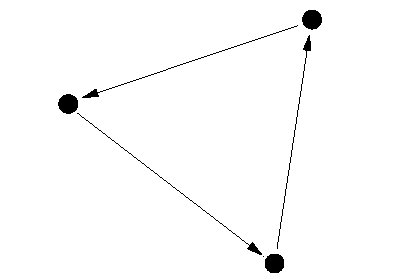
\includegraphics{./sci-pap-roc.pdf}%
\end{picture}%
\setlength{\unitlength}{3947sp}%
%
\begingroup\makeatletter\ifx\SetFigFont\undefined%
\gdef\SetFigFont#1#2#3#4#5{%
  \reset@font\fontsize{#1}{#2pt}%
  \fontfamily{#3}\fontseries{#4}\fontshape{#5}%
  \selectfont}%
\fi\endgroup%
\begin{picture}(3345,2223)(3054,-2286)
\put(5469,-1199){\makebox(0,0)[lb]{\smash{{\SetFigFont{12}{14.4}{\familydefault}{\mddefault}{\updefault}{\color[rgb]{0,0,0}smashes}%
}}}}
\put(5723,-213){\makebox(0,0)[lb]{\smash{{\SetFigFont{12}{14.4}{\familydefault}{\mddefault}{\updefault}{\color[rgb]{0,0,0}scissors}%
}}}}
\put(5381,-2271){\makebox(0,0)[lb]{\smash{{\SetFigFont{12}{14.4}{\familydefault}{\mddefault}{\updefault}{\color[rgb]{0,0,0}rock}%
}}}}
\put(3956,-1652){\makebox(0,0)[lb]{\smash{{\SetFigFont{12}{14.4}{\familydefault}{\mddefault}{\updefault}{\color[rgb]{0,0,0}covers}%
}}}}
\put(4423,-463){\makebox(0,0)[lb]{\smash{{\SetFigFont{12}{14.4}{\familydefault}{\mddefault}{\updefault}{\color[rgb]{0,0,0}cuts}%
}}}}
\put(3069,-837){\makebox(0,0)[lb]{\smash{{\SetFigFont{12}{14.4}{\familydefault}{\mddefault}{\updefault}{\color[rgb]{0,0,0}paper}%
}}}}
\end{picture}%

\end{center}
  
\hint{If at first you don't succeed\ldots \newline
try googling ``scissor paper rock lizard spock.''}

\wbvfill

\workbookpagebreak

\end{enumerate}




%\newpage
%\renewcommand{\bibname}{References for chapter 3}
%\bibliographystyle{plain}
%\bibliography{main}

%% Emacs customization
%% 
%% Local Variables: ***
%% TeX-master: "GIAM.tex" ***
%% comment-column:0 ***
%% comment-start: "%% "  ***
%% comment-end:"***" ***
%% End: ***
 
